%!TEX program = xelatex
%!TEX TS-program = xelatex
%!TEX encoding = UTF-8 Unicode

% 项目地址:https://gitee.com/hrrcn/BjutThesisTemplate.git
% type参数为学位类型,bachelor|master|doctor|postdoctor
% 专硕使用参数professional,学硕去掉此参数。
% 若无法编译加粗字体,添加参数AutoFakeBold;否则去掉参数。
\documentclass[type=master,professional,AutoFakeBold=0.5]{bjutthesis}
% 引用自定义的bjutthesis.cls类文件 %
\usepackage{bjutthesis}
% 正文中插入代码包 %
\usepackage{listings}
%\usepackage{caption}
% 表格单元格设置包 %
\usepackage{makecell}
% 禁止图片和表格浮动
% 用法:\begin{figure}[H]
%      \begin{table}[H]
\usepackage{float}
\usepackage{longtable}

%
% 代码段引用设置
%
%\setmonofont{Consolas}
%\setmonofont{Courier New}
\lstset{
 %basicstyle=\fontspec{SimHei},
 %basicstyle=\ttfamily,
 %basicstyle=\sffamily,   %\footnotesize \sffamily,
 breaklines=true,                                    %这条命令可以让LaTeX自动将长的代码行换行排版
 %extendedchars=true,                                %解决代码跨页时,章节标题,页眉等汉字不显示的问题
 %columns=fixed,       
 %numbers=left,                                      % 在左侧显示行号
 %numberstyle=\tiny\color{gray},                     % 设定行号格式
 %frame=shadowbox,                                   % 显示背景边框
 %backgroundcolor=\color[RGB]{245,245,244},          % 设定背景颜色
 keywordstyle=\color[RGB]{40,40,255},                % 设定关键字颜色
 %numberstyle=\footnotesize\color{darkgray},           
 %commentstyle=\it\color[RGB]{0,96,96},              % 设置代码注释的格式
 %commentstyle=\it\color{red!50!green!50!blue!50},
 %stringstyle=\rmfamily\slshape\color[RGB]{128,0,0}, % 设置字符串格式
 showstringspaces=false,                             % 不显示字符串中的空格
 %language=c,                                        % 设置语言
 flexiblecolumns,                                    % 自动调整字间距
}

% 定义所有的图片文件在fig子目录下 %
\graphicspath{{fig/}}

%
% 设置封面
%
\begin{document}
\frontmatter
%封面与摘要中英文
\thusetup{
  udc={004}, %无需修改
  id={10005},%无需修改
  secretlevel={公开},%无需修改
  catalognumber={TP391.1}, %无需修改
  % ccovertype={硕\hspace{\fill}士\hspace{\fill}学\hspace{\fill}位\hspace{\fill}论\hspace{\fill}文},  % 彩色封面标题,学硕
  ccovertype={硕\hspace{\fill}士\hspace{\fill}专\hspace{\fill}业\hspace{\fill}学\hspace{\fill}位\hspace{\fill}论\hspace{\fill}文}, % 彩色封面标题,专硕
  % cthesistype={北京工业大学工学硕士学位论文}, % 内封面标题,学硕
  cthesistype={北京工业大学硕士专业学位论文}, % 内封面标题,专硕
  %cthesistypep={(非全日制)}, % 内封面标题,全日制或非全日制或同等学力等。学硕请忽略。
  % cpageheading={北京工业大学工学硕士学位论文}, % 页眉,学硕
  cpageheading={北京工业大学工程硕士专业学位论文}, % 页眉,专硕
  cstudent={S201861807},
  ctitle={基于UEFI的硬盘文件安全加载策略研究与实现},
  cauthor={唐治中},
  cdepartment={计算机技术},
  cmajor={信息安全},
  cdegree={工程硕士专业学位},
  csupervisor={张建标\ \ 教授},
  ccollege={信息学部计算机学院},  
  cdate={2021年6月},
  corganization={北京工业大学},
  %
  %=========
  % 英文信息
  %=========
  % ecovertype={MASTERAL\  DISSERTATION}, % 学硕
  ecovertype={PROFESSIONAL\  master\  DISSERTATION}, % 专硕
  etitle={Research and Implementation of Hard Disk File Security Loading Strategy Based on UEFI},
  edegree={Master of Engineering},
  emajor={Computer Science and Technology},
  eauthor={Tang Zhizhong},
  esupervisor={Associate Professor Wei Ma}
}

% 定义中英文摘要和关键字
% 摘要中文大致一页长度 一段背景引入本文研究 说现有问题总结 本文贡献主要创新点 3个研究内容 3个创新点
\begin{cabstract}

随着科学的发展,技术的进步,越来越多的计算机上层应用得到极大的发展,例如人工智能和区块链、物联网等,而这些
技术的发展和流行,都要依赖于操作系统或更底层系统的功能支持和安全保障。《信息安全技术 网络安全等级保护基本要求》
国家标准中就指出,实际运行中的关键系统需要进行各阶段的可信验证工作。UEFI规范作为近些年来替代传统BIOS的一种
底层系统规范,从各个机构的服务器到每个人的个人计算机,都得到了广泛的应用。UEFI BIOS在可扩展性和开发效率、开发
难易程度上都得到极大的增强,但正是这种C语言来替代传统汇编语言的方案,使得UEFI BIOS同样会遭受C语言代码的攻击,
不同处理器架构的统一规范开发方式也为攻击底层固件系统提供了更多的条件。从硬盘这样的块设备经过UEFI BIOS启动操作
系统仍然是如今主流的系统启动方式,他涉及到的不光是硬盘设备的被攻击的可能性,也涉及到固件系统层面的攻击,如对于
UEFI文件系统这样的操作硬盘的内部逻辑,就更易收到针对性的攻击对硬盘文件的安全性带来威胁。因此研究基于UEFI的硬盘
文件的安全加载就具有重要意义。本文主要工作如下:
\par (1)针对UEFI BIOS系统加载硬盘文件过程中存在的安全威胁,通过研究硬盘设备用于存放UEFI BIOS环境中可访问数据的
ESP分区的组织结构,研究UEFI BIOS环境中读取硬盘文件的方式,以及研究以UEFI型驱动程序作为基础的可信度量机制,以此
确保针对硬盘设备攻击的文件安全性。结合可信计算理论提出基于UEFI的硬盘设备文件可信加载的总体框架,研究解决UEFI BIOS
环境加载硬盘文件过程中的安全可信。
\par (2)针对UEFI BIOS系统的启动阶段设计,通过研究各个阶段的加载功能和特点,结合可信计算技术,确定每个阶段
需要度量的固件芯片中的代码内容,以UEFI启动的第一阶段作为整个系统的可信根,逐个度量后面阶段的核心代码,将信任链
逐阶段传递,一直到UEFI加载硬盘文件的BDS阶段,以保证加载文件前,系统的安全可信性。
\par (3)针对系统中使用的可信计算平台,设计出以BMC系统作为可信平台的方案,通过特定的BMC通信协议和接口对其
进行通信功能的开发,并根据UEFI启动阶段的特性,设计出PEI阶段和DXE阶段分别开发BMC驱动程序的方案,来达到各个
阶段度量特定驱动和代码的效果。
\par 

\end{cabstract}

\ckeywords{UEFI, 文件系统协议栈, BMC, 可信计算, 信任链}

\begin{eabstract}

With the development of science and technology, more and more computer upper-level applications 
have been greatly developed, such as artificial intelligence, blockchain, and the Internet of Things. 
The development and popularity of these technologies depend on operating systems. Or the functional 
support and security guarantee of the lower-level system. According to the national standard of 
"Information Security Technology Network Security Graded Protection Basic Requirements", critical 
systems in actual operation need to be trusted at various stages. As a low-level system specification 
that replaces traditional BIOS in recent years, UEFI specification has been widely used from servers 
of various organizations to personal computers of everyone. UEFI BIOS has been greatly enhanced in 
terms of scalability, development efficiency, and development difficulty. However, it is this C 
language that replaces the traditional assembly language program, which makes UEFI BIOS also subject 
to C language code attacks. The unified specification development method of the processor 
architecture also provides more conditions for attacking the underlying firmware system. 
Starting the operating system from a block device such as a hard disk through UEFI BIOS is 
still the mainstream system startup method today. It involves not only the possibility of the 
hard disk device being attacked, but also the firmware system level attack, such as the UEFI 
file system. Such internal logic of operating the hard disk makes it easier to receive 
targeted attacks that threaten the security of hard disk files. Therefore, it is of great 
significance to study the secure loading of UEFI-based hard disk files. The main work of this 
paper is as follows:
\par (1)In view of the security threats in the process of loading hard disk files in the UEFI 
BIOS system, the organization structure of the ESP partition of the hard disk device used to store 
the accessible data in the UEFI BIOS environment is studied, the method of reading hard disk files 
in the UEFI BIOS environment, and the research UEFI-type drivers are used as the basic credibility 
measurement mechanism to ensure file security against hard disk device attacks. Combining with 
the theory of trusted computing, a general framework for trusted loading of hard disk device files 
based on UEFI is proposed, and the security and trustworthiness of the process of loading hard 
disk files in the UEFI BIOS environment is studied.
\par (2)Aiming at the design of the boot phase of the UEFI BIOS system, by studying the loading 
functions and characteristics of each phase, combined with trusted computing technology, determine 
the code content in the firmware chip that needs to be measured at each phase, and the first phase 
of UEFI boot as the entire system The root of trust measures the core code of the later stages 
one by one, and passes the chain of trust stage by stage until the BDS stage of UEFI loading hard 
disk files to ensure the security and credibility of the system before loading files.
\par (3)Aiming at the trusted computing platform used in the system, the BMC system is designed 
as a trusted platform, and the BMC communication protocol and interface
Carry out the development of communication functions, and according to the characteristics of the 
UEFI boot phase, design the PEI phase and the DXE phase to develop the BMC driver program separately 
to achieve each Phase measures the effect of specific drivers and codes.

\end{eabstract}

\ekeywords{UEFI, File system protocol stack, BMC, trusted computing, Chain of trust}

\makecover

%
% 目录
%
\tableofcontents
% 保证在偶数页结束本章节 %
\bjutclearpage

%% 插图索引
%\listoffigures
%\bjutclearpage

%% 表格索引
%\listoftables
%\bjutclearpage

%% 公式索引
%\listofequations
%\bjutclearpage

%% 符号表示 
%% 写法一,单列列表,可以通过参数设置label宽度
% \begin{denotation} % [5cm]
%     \item[E] 误差
%     \item[T] 位姿
%     \item[$\bm{P}$] 三维点
% \end{denotation}  
% 写法二,两列表格,可以通过参数做单列或加三线等,参数格式同tabular
\begin{notation}%[p{1.4cm}<{\centering} p{5cm}<{\centering} p{1.4cm}<{\centering} p{5cm}<{\centering}]
    \hline
    符号 &含义 &
    符号 &含义\\
    \hline
    $\bm{P}$ &三维点 &        
    $\bm{L}$  &三维线\\
    $\bm{p}$ &二维点 &
    $\bm{l}$ &二维线\\
    $\bm{\pi}$ &平面 &
    $F$ &图像帧 \\
    $\bm{R}$ &旋转矩阵 &
    $\bm{t}$ &平移向量 \\
    $\bm{K}$  &相机内参矩阵 &       
    $\bm{T}$ &相机变换矩阵 \\
    $\bm{\mathcal{K}}$ & 直线投影的相机内参矩阵 &
    $\bm{\mathcal{H}}$ & 三维直线的相机变换矩阵 \\
    $\rho_h$ &Huber鲁棒代价函数 &       
    $\phi$ &投影函数\\
    $e$ &重投影误差 &
    $E$     &误差函数 \\
    $\bm{\Omega}$ &协方差矩阵 &
    $\Phi$ & 可信度 \\
    \hline
\end{notation}
%\bjutclearpage

%
% 正文部分
%
\mainmatter
%
% 第一章
%
\chapter{绪论}
%
% 2.1节
%
\section{背景及研究意义}
目前,在计算机应用领域,统一可扩展固件接口UEFI(Unified Extensible Firmware Interface)
已经成为了主流基础输入输出系统BIOS(Basic Input/Output System)实现方式并
逐渐取代了传统BIOS,作为一个越来越成熟的BIOS系统,UEFI环境就包括了对硬盘文件加载和运行的功能,其中包括:在调试
关键驱动程序时,可能需要把驱动文件放入硬盘并在UEFI SHELL环境中手动加载\cite{english16,english20};
操作系统启动需要经过UEFI环境,并在其中加载硬盘中
的操作系统引导程序完成启动,也包括UEFI远程安装并启动操作系统的功能\cite{chinese29}。
在UEFI初始化完成后,可完整使用UEFI提供的系统功能,其中就包括了硬盘中的可扩展固件接口
文件系统分区ESP(Efi system partition)分区数据操作。这块UEFI可访问到的硬盘空间上会存储一些UEFI编译
过程中重要的可扩展固件接口
可执行文件.efi文件,其中就包括了操作系统启动引导文件start\_kernel.efi这样的关键文件\cite{chinese18},
因此如何在UEFI环境中安全的加载硬盘设备文件就成了关键问题。
\par 因为在UEFI环境下访问硬盘文件,所以这些文件存在通过硬盘被篡改和通过UEFI文件系统被篡改的可能性
\cite{chinese16}。现有技术中有针
对硬盘文件的硬件攻击方法\cite{english5},通过硬件手段修改硬盘中关键文件的内容起到注入木马程序的效果。
还有一种现有技术中针对存
放BIOS程序的闪存flash芯片提出了一种攻击手段,其攻击原理为通过硬件手段和flash中数据存储格式,修改flash
芯片中的驱动程序内容起到注入木马程序的效果。因为UEFI中访问硬盘文件需要经过UEFI文件系统协议栈,因此通过现有技
术手段可修改协议栈相关驱动\cite{english3},从UEFI固件层面达到攻击效果。因此对于BIOS固件层面的块设备文件
系统的可信验证是极其具有必要性的\cite{english17,english6,english7}。

%
% 2.2节
%
\section{国内外研究现状}
房强等在“基于固件文件系统的UEFI安全机制研究”一文中通过对UEFI安全威胁研究的分析与总结\cite{chinese11},提出了基于可信平台模块TPM
(下同)的静态度量固件文件系统中驱动程序的方法。该方案以TPM为可信锚点,此信任根可根据如基板管理控制器BMC(下同)
这样的底层硬件进行替代和改进;其次对于固件文件系统FFS(下同)中的驱动文件度量为静态度量过程,及在UEFI初始化阶段
结束后再进行度量,这样就无法保证初始化过程中的安全性。段晨辉等在“UEFI BIOS安全增强机制及完整性度量的研究“
\cite{chinese8}一文中
通过对UEFI启动阶段中信任链的设计和底层基于可信计算组织TCG(下同)的可信链构建方案,提出了在UEFI完整启动阶段过程
中通过逐个阶段度量后面阶段的内容起到可信启动的效果。但该方案在整个度量过程中需要涉及到驱动加载准备阶段PEI阶段
(下同)核心代码、所有PEI模块程序、驱动加载阶段DXE(下同)核心代码、DXE调度器代码、所有DXE驱动程序代码的度量
工作,缺少对于特定如硬盘设备文件的文件系统的针对性安全验证,并且整个度量过程繁琐耗时,虽然做到了动态度量效果,
但具有相当大的局限性,可行性不高。
\par 文献\mcite{chineses36}提出了一种通过
UEFI固件层面的文件安全存储策略,来保证硬盘文件受到攻击和恶意篡改时可通过BIOS固件中的文件信息进行复原。但是该
专利忽略了对于固件硬件平台的攻击可能性,无法保证固件中备份文件的安全性,即文件的硬件安全防护能力并不突出。
文献\mcite{chineses35}提出了一种通过检测硬盘设备是否安
全可信的机制完成硬盘文件的安全加载。但是该方案忽略了通过篡改BIOS固件中文件系统相关驱动达到修改硬盘文件的手段,
一旦固件中的文件系统被恶意篡改,在UEFI环境中加载硬盘文件不存在可信而言。
\par 在UEFI安全领域\cite{english9,english10,english11},
大部分基于UEFI的文件加载方案,没有对固件层面的UEFI文件系统驱动可信度量的过程,无法保证固件层面针对硬盘文件
内容的攻击。一些完整性度量方案中着重度量系统的全部信息,缺少一些针对性的驱动内容的度量工作\cite{english4}。
\par 现有研究中也有通过USB Key的方式存储操作系统引导文件\cite{english15},避免了计算机硬盘被攻击的可能,
但USB设备仍然属于块设备硬件,也存在被攻击的风险。UEFI系统的可信启动也成了近年来重点研究的对象\cite{english8,english14}
,从UEFI启动的各个阶段逐一度量后一阶段然后进行控制权的传递。随着国产化的流行\cite{english19},同时也为了
适应各种国产硬件如CPU等设备的适配,UEFI的国产化研究适配工作也急需进行。

%
% 2.3节
%
\section{主要研究内容}
鉴于UEFI是BIOS系统的一种统一可扩展标准和方案,拥有着模块化的系统部件添加结构,使他成为BIOS功能开发的首选方案,
目前市场上的BIOS实现也越来越多的统一使用UEFI。与此同时,UEFI BIOS作为计算机启动到加载操作系统的一个中间阶段,
需要在系统启动时加载硬盘中ESP分区中的操作系统引导程序;并且随着UEFI BIOS的功能的不断发展,UEFI BIOS环境中甚至
能够播放视频音频,而硬盘设备又是计算机中数据的主要存储介质,这就增加了BIOS与硬盘设备之间交互频率\cite{chinese10},BIOS环境中
加载硬盘设备文件的安全性就显得更加重要。因此研究基于UEFI的硬盘设备文件加载的安全机制就具有重要意义。
\par 本文主要研究内容如下:
% \par (1)针对UEFI BIOS系统加载硬盘文件过程中存在的安全威胁,通过研究硬盘设备用于存放UEFI BIOS环境中可访问数据的
% ESP分区的组织结构,研究UEFI BIOS环境中读取硬盘文件的方式,以及研究以UEFI型驱动程序作为基础的可信度量机制,以此
% 确保针对硬盘设备攻击的文件安全性。结合可信计算理论提出基于UEFI的硬盘设备文件可信加载的总体框架,并使用的底层可信
% 平台BMC及基板管理控制器,研究UEFI BIOS中BMC驱动程序的实现原理及具体
% 过程,研究UEFI BIOS和BMC如何通过基础驱动程序构建安全方案中取得基准值及度量报告的写入方法,以此确保BMC作为本
% 系统安全方案的可信平台为UEFI提供服务,研究解决UEFI BIOS环境加载硬盘文件过程中的安全可信。
\par (1)针对UEFI BIOS系统加载硬盘文件过程中存在的安全威胁,结合可信计算理论提出基于UEFI的硬盘设备文件可信
加载的总体框架,并使用的底层可信平台BMC及基板管理控制器,实现UEFI BIOS中BMC驱动程序。
% \par (2)针对UEFI BIOS系统加载UEFI BIOS存储闪存设备中的驱动文件过程中存在的安全问题,研究作为UEFI BIOS中最为
% 关键的系统组件UEFI驱动程序在闪存介质中的数据存储格式,研究PEI和DXE两个加载UEFI驱动程序的主要启动阶段的具体驱动
% 加载流程和原理,研究可信度量功能在这两个主要阶段中的构建位置。以此确保针对BIOS闪存攻击硬盘文件系统程序(以达到
% 在BIOS加载硬盘文件时篡改文件内容的目的)过程的安全性。
\par (2)针对UEFI BIOS系统加载UEFI BIOS存储闪存设备中的驱动文件过程中存在的安全问题,设计提出UEFI BIOS启动
阶段所需度量的UEFI文件系统协议栈驱动程序,并实现度量模块功能。
% \par (3)针对安全方案中的驱动加载、度量和日志存储功能,研究UEFI环境下DXE阶段的依赖表达式,来达到修改驱动加载顺序
% 以保证在被度量驱动加载前加载可信度量驱动程序的目的。研究申威真机环境下通过IO端口映射的方式向BMC发送度量日志,
% 并且根据UEFI规范找到匹配特定驱动并对其进行度量的方法。
\par (3)针对安全方案中的可信度量功能,设计并实现了通过BMC的日志存储功能,并完成确保驱动按顺序加载的依赖表达式
编写。
\par (4)根据本系统安全方案的设计,在申威平台中对驱动度量模块、日志生成功能和驱动加载
顺序修改功能进行实现和测试,以保证功能开发过程的有效性和安全方案的可实施性。

%
% 2.4节
%
\section{本文组织结构}
全文结构一共分为六大部分,各部分内容如下:
\begin{itemize}
\item 第一章\quad 绪论
\par 首先对本文的研究背景和研究意义进行了介绍,然后阐述了现有的UEFI环境下硬盘文件保护方法的
现状及本系统在这个基础上做的改进。介绍了本文的主要研究内容,最后介绍了本文的组织结构。
\item 第二章\quad 相关知识及技术介绍
\par 首先对UEFI BIOS及可扩展固件接口标准的基础输入输出系统的整体设计和层次结构进行了介绍,包括
启动流程、协议加载方式、数据库句柄及固件文件系统数据存储格式。其次对UEFI文件系统协议栈及涉及到的具体
驱动程序做了进一步说明。然后介绍了BMC及基板控制管理器的基本功能及与BIOS通信方式。最后介绍了可信计算技术
的现状及发展。
\item 第三章\quad 基于UEFI的硬盘文件安全加载系统总体设计
\par 首先对UEFI环境中加载硬盘文件的安全漏洞进行了分析,其次介绍了此系统中信任链的涉及与传递,
然后介绍了系统的总体架构设计,包括了DXE和运行时两个主要的度量阶段。最后介绍了此系统的功能模块划分。
\item 第四章\quad 基于UEFI的硬盘文件安全加载系统详细设计
\par 分别对度量计算模块、硬盘文件度量模块、驱动文件度量模块、固件和硬盘访问模块、
BMC通信模块给出了具体设计和关键代码实例,并对SEC、PEI和DXE阶段做了补充说明。
\item 第五章\quad 硬盘文件可信加载方案实现及测试
\par 根据此系统的安全方案设计,介绍了如BMC驱动、文件系统相关驱动的实现、实验及测试过程,以及实验相关的编译
运行环境。通过实验说明了安全方案的可实施性和此系统的预防效果。
\item 结论
\par 对本文的相关研究工作进行了总结和分析,并根据功能测试结果指出本方案的不足之处。并提出了下
一步的研究方向。
\end{itemize}

%
% 第二章
%
\chapter{相关知识及技术介绍}

%
% 2.1节
%
\section{UEFI概述}
本章将会介绍UEFI系统中关系到本文关键技术的基础内容,其中具体包括了UEFI基本结构、UEFI固件存储格式、
UEFI文件系统协议栈相关内容及驱动程序介绍,还包括基板管理控制器BMC及可信计算的基础内容。

\subsection{UEFI系统结构}
UEFI(Unified Extensible Firmware Interface,统一可扩展固件接口)定义了操作系统和平台固件直接的接口,
UEFI 提供了一个统一可扩展的固件平台,并针对平台特性定义了一系列接口。该平台整体处于硬件与操作系统中间,
平台最上层的可扩展固件接口包含了平台提供的 API 函数、启动时服务(EFI  Boot  Services)、运行时服务
(EFI  Runtime Services)和操作系统引导程序\cite{english21},下层则是根据 UEFI 规范实现的平台固件。
UEFI的平台架构
如图 2-1 所示:

\begin{figure}[htb]
    %\label{infrastructure_of_uefi}
    % 调整图片与上文的垂直距离 %
    \vspace{0cm}
    % 调整图片图片与中文标题、中文标题与英文标题距离 % 
    \setlength{\abovecaptionskip}{0.3cm}
    % 引用/fig/目录中的图片文件 %
	\centering
    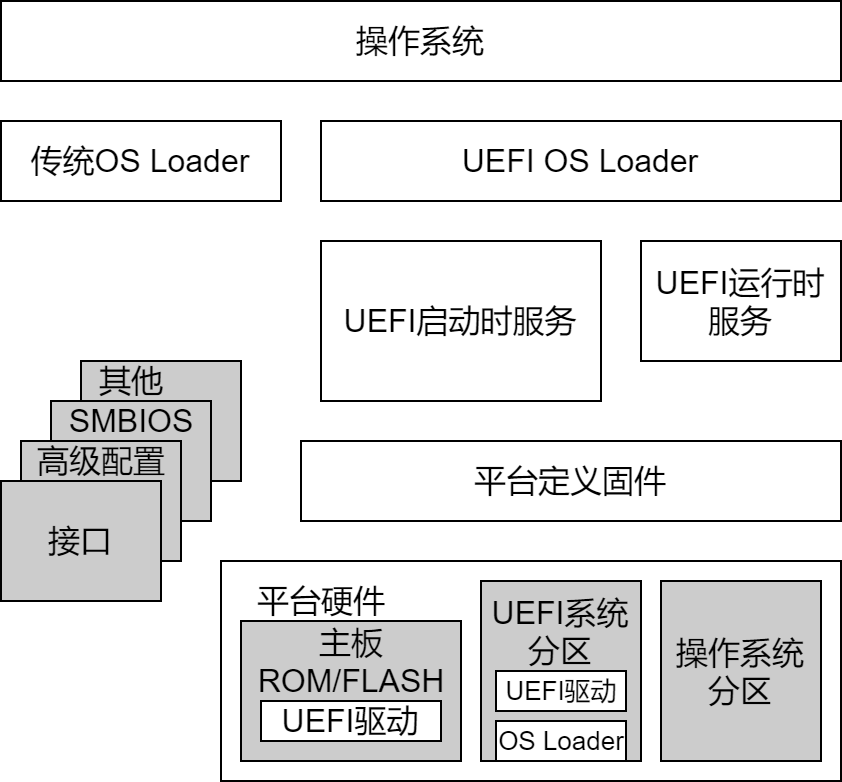
\includegraphics[width=8cm]{infrastructure_of_uefi2.png}
    % 中文标题 %
    \caption*{图 2-1 UEFI系统框架图}
    % 调整图片英文标题与下文距离 %
    \setlength{\belowcaptionskip}{-0.7cm}
    % 英文标题 %
    \caption*{Figure 2-1 Infrastructure of UEFI}
\end{figure}

\par 图 2-1 描绘了UEFI框架中各模块的关系,UEFI固件作为承上启下的模块,对底层硬件进行了抽象处理,
又不断地对上层的操作系统提供服务,并在不同的服务层的连接中采用了标准的接口。图中UEFI保留了对
传统BIOS引导操作系统的兼容性,所以在可扩展固件接口的实现中有两种操作系统引导方式,分别为
Legacy OS Loader 和UEFI OS Loader。 
\par UEFI允许操作系统预处理,实现了操作系统的引导和一些系统软件执行所需要的其它应用程序,
如诊断程序、UEFI Shell、系统调试软件等,这些程序统称为UEFI实体(UEFI Image)。根据UEFI规范,
UEFI Image包含三种:UEFI应用程序、UEFI驱动和OS Loaders,这些实体都是在UEFI API调用的基础上
实现的。
\par 从图中可以看出,UEFI的启动时服务Boot Service中包含了UEFI在PEI和DXE两个主要加载驱动完成
系统初始化过程中所需要的驱动程序、内存管理、设备管理、协议贮存等信息。而UEFI的启动时服务也有他
自己的生命周期,从下图就可以看出启动时服务在UEFI启动过程中的位置。

\begin{figure}[htb]
    %\label{bootint_sequence}
    % 调整图片与上文的垂直距离 %
    \vspace{0cm}   
    % 调整图片图片与中文标题、中文标题与英文标题距离 %                             
    \setlength{\abovecaptionskip}{0.3cm}  
    % 引用/fig/目录中的图片文件 %
	\centering
    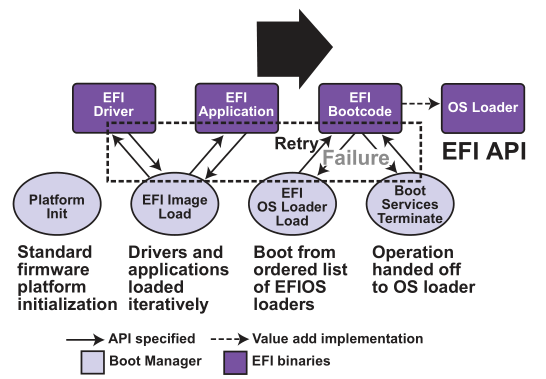
\includegraphics[width=10cm]{boot_seq.png}
    % 中文标题 %
    \caption*{图 2-2 统一可扩展固件接口启动流程图}
    % 调整图片英文标题与下文距离 %
    \setlength{\belowcaptionskip}{-0.7cm}
    % 英文标题 %
    \caption*{Figure 2-2 Booting Sequence of UEFI}
\end{figure}

从图2-2中可以看出,Platform Init平台初始化过程中建立Boot Service系统服务和RunTime Service系统服务,
EFI Image Load阶段包括了
PEI和DXE两个主要驱动加载过程,负责加载BIOS固件中的UEFI驱动和UEFI应用程序的EFI可执行文件,之后在启动
设备选择也就是BDS阶段中,通过用户的选择,UEFI BIOS选择适当的操作系统引导程序进行加载,并同时退出
Boot Service服务,并继续向上层操作系统提供RunTime Service服务。因而在操作系统运行过程中,可以继续使
用底层UEFI BIOS提
供的运行时服务。结合图2-1也可以发现,UEFI的一些关键驱动程序,和OS Loader也会存放在如硬盘块设备的ESP
(EFI System Partition)系统分区中。由于本文主要对于UEFI启动过程中的DXE、BDS阶段进行安全方案设计,
因此,启动时服务其中包含的如协议加载函数等为本文的主要研究对象。

\subsection{UEFI协议运作方式}
UEFI中协议设计的思想为,由于UEFI的官方提供实现的版本为C语言实现,而C语言是一种面向过程的语言,而完全
使用面向过程的思想来管理和使用众多UEFI协议将会使程序变得非常复杂。Protocol作为一种对象来设计管理会更加
直观\cite{english13,english12}。因而UEFI中的Protocol引入了面向对象的思想,其中包括:
\begin{itemize}
\item 用struct来模拟class。
\item 用函数指针(Protocol的成员变量)模拟成员函数,此种函数的第一参数必须是指向Protocol的指针,用来
模拟this指针。
\end{itemize}
\par 从图2-1中可以看出,UEFI中的协议包含于UEFI启动时服务中(Boot Services),由启动时服务提供的功能进行
协议的加载、保存和调用等操作。其中UEFI启动时服务提供的协议相关的功能函数如表2-1所示。

\begin{table}[htb]
    %\label{tab:parametervalues}
    % 设置表内行间距 %
    \renewcommand\arraystretch{1.5}
    % 设置表题目 %
	\caption*{表 2-1 启动时服务协议功能表}
	\caption*{Table 2-1 Boot Service Protocol Interface Functions}
    \begin{tabular*}{\hsize}{@{}@{\extracolsep{\fill}}ccl@{}}
    % 表上线和表头 %
	\toprule[0.75pt]
    名称  &类型  &\makecell[c]{描述}\\
    % 表中线和表内容 %
	\midrule[0.5pt]
	InstallProtocolInterface   &Boot  &\quad 在设备句柄上安装一个协议接口\\
    UninstallProtocolInterface &Boot  &\quad 从设备句柄上移除一个协议接口\\
    ReinstallProtocolInterface &Boot  &\quad 在设备句柄上重新安装协议接口\\
    RegisterProtocolNotify     &Boot  &\makecell[l]{ 
                                       \quad 注册一个事件,只要接口有信号为指定的\\
                                             协议安装\\
                                        }\\
    LocateHandle               &Boot  &\quad 返回支持指定协议的句柄数组\\
    HandleProtocol             &Boot  &\quad 查询句柄以确定它是否支持指定的协议\\
    LocateDevicePath           &Boot  &\makecell[l]{
                                       \quad 找到支持指定路径的设备路径上的所有设\\
                                             备协议并将句柄返回到最接近的设备路径
                                        }\\
    OpenProtocol               &Boot  &\quad 将元素添加到使用协议的代理列表中接口\\
    CloseProtocol              &Boot  &\makecell[l]{
                                       \quad 从代理列表中移除一个元素,也就是消耗\\
                                             一个协议接口
                                        }\\
    OpenProtocolInformation    &Boot  &\quad 检索当前正在使用的代理列表协议接口\\
    ConnectController          &Boot  &\makecell[l]{
                                       \quad 使用一组优先规则来找到最佳的驱动程序\\
                                             集管理一个控制器
                                        }\\
    DisconnectController       &Boot  &\quad 通知一组驱动程序以停止管理控制器\\
    ProtocolsPerHandle         &Boot  &\makecell[l]{
                                       \quad 检索安装在句柄上的协议列表,函数返回\\
                                             的缓冲区是自动分配的
                                        }\\
    LocateHandleBuffer         &Boot  &\makecell[l]{
                                       \quad 从句柄数据库中检索句柄列表,该列表符\\
                                             合搜索条件,返回缓冲区自动已分配
                                        }\\
    LocateProtocol             &Boot  &\makecell[l]{
                                       \quad 在句柄数据库中找到第一个支持所需协议\\
                                             的句柄\\
                                        }\\
    InstallMultipleProtocolInterfaces
                               &Boot  &\quad 将一个或多个协议接口安装到指定句柄上\\
    UninstallMultipleProtocolInterfaces
                               &Boot  &\quad 从指定句柄中卸载一个或多个协议接口\\
    % 表下线 %
	\bottomrule[0.75pt]
    \end{tabular*}
    % 表格与下文距离 %
	\vspace{-0.3cm}
\end{table}

表2-1中列出了Boot Service中包含的所有UEFI协议相关的功能函数,其中最为常见的如InstallMultip
leProtocolInterfaces这样的加载协议函数,在众多UEFI应用以及底层驱动程序中都十分常见,因为他
可以同时提供出需要加载的多个协议GUID。
\par 同时,由于启动时服务提供了追踪最新安装了的新协议内容以及他们的使用情况,因此对于UEFI的启动时服务
来说,它可以安全地卸载并重新安装由UEFI驱动程序使用的协议接口。

\begin{figure}[htb]
    %\label{bootint_sequence}
    % 调整图片与上文的垂直距离 %
    \vspace{0cm}   
    % 调整图片图片与中文标题、中文标题与英文标题距离 %                             
    \setlength{\abovecaptionskip}{0.3cm}  
    % 引用/fig/目录中的图片文件 %
	\centering
    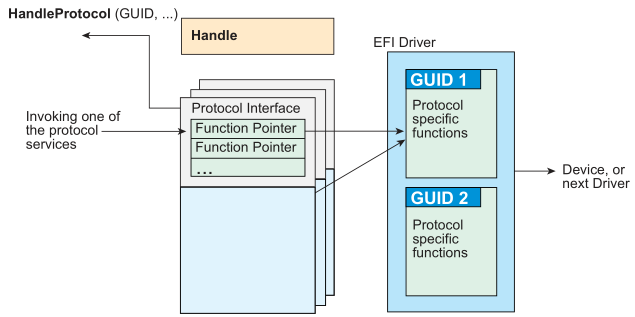
\includegraphics[width=10cm]{locate_protocol.png}
    % 中文标题 %
    \caption*{图 2-3 统一可扩展固件接口协议加载方式图}
    % 调整图片英文标题与下文距离 %
    \setlength{\belowcaptionskip}{-0.7cm}
    % 英文标题 %
    \caption*{Figure 2-3 Locating Protocol of UEFI}
\end{figure}

\par 协议的加载过程可通过图2-3分析得知。在图2-3中可以看出,协议由HandleProtocol等表2-1中列出的装载协议
用的功能函数加载到Handle句柄上,而所有的Handle则由UEFI内核统一存储于句柄数据库,句柄数据库也是一个链表
结构用于存储记录所有的Handle句柄,这些句柄可由任意的UEFI Image(镜像)访问,从而达到函数调用的效果。而这
些协议中包含的是指向具体函数的C语言中的函数指针,这些具体函数则是在DXE阶段由UEFI系统表提供的加载驱动镜像函数
加载并驻留在内存中的。

%
% 2.2节
%
\section{UEFI固件文件系统数据存储方式介绍}
UEFI固件文件系统指的是BIOS闪存芯片中的数据存储格式,它通过统一的固件文件系统标准用来统一闪存芯片中的文件
内容和UEFI启动阶段内存中文件的内容\cite{chinese21}。具体的固件中UEFI可执行程序文件存储格式如图2-4所示。

\begin{figure}[htb]
    %\label{ffs_format}
    % 调整图片与上文的垂直距离 %
    \vspace{0cm}   
    % 调整图片图片与中文标题、中文标题与英文标题距离 %                             
    \setlength{\abovecaptionskip}{0.3cm}  
    % 引用/fig/目录中的图片文件 %
	\centering
    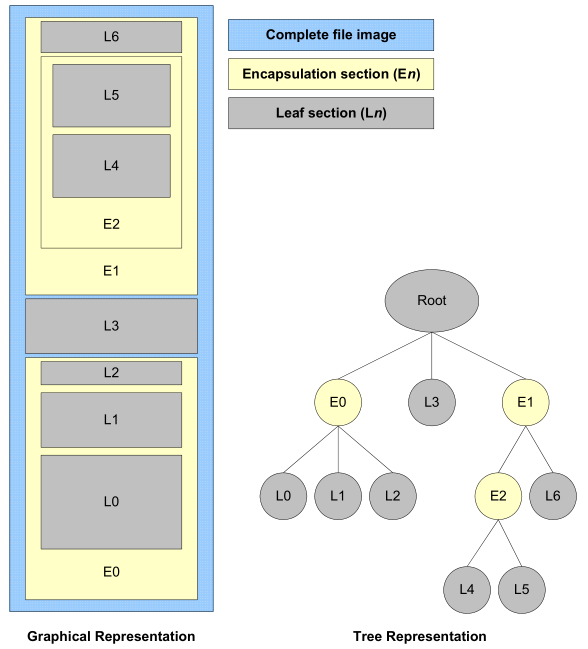
\includegraphics[width=10cm]{ffs_struct.PNG}
    % 中文标题 %
    \caption*{图 2-4 固件文件系统文件存储格式}
    % 调整图片英文标题与下文距离 %
    \setlength{\belowcaptionskip}{-0.7cm}
    % 英文标题 %
    \caption*{Figure 2-4 Firmware file system file storage format}
\end{figure}

在图2-4中,左边为通过结构图的方式说明固件文件系统的数据存储格式,右边为通过数据结构中的树形结构来阐述
FFS中的文件存储。右图中,蓝色方框代表了一个完整的FFS中的文件映像也就是UEFI中可执行文件的二进制数据,
黄色方框代表了一个父目录结构,黄色方框中包含的灰色方框代表了父目录中的子目录,也就是文件影响中的最小
单位。对应到右图的树结构中,黄色节点就是树中有子节点的父节点,而灰色节点则代表了叶子节点。了解固件文件
系统中的文件数据存储格式有助于理解UEFI内核在系统初始化过程中调用相关解析FFS中文件函数的运行过程,也有
助于帮助分析本文安全方案中可信度量的具体数据内容。
%
% 2.3节
%
\section{UEFI文件系统协议栈}
UEFI BIOS中的文件系统协议栈指的是针对块设备,也就是对应一般应用于PC和服务器上的硬盘设备,UEFI文件
系统协议栈通过把对硬盘设备的不同操作功能分层起到区分和满足应用层与内核层不同功能需要的目的,下面本
节将做具体的介绍。
\subsection{总体介绍}
UEFI BIOS和传统BIOS都支持硬盘的读写功能。UEFI优于传统BIOS的地方在于,UEFI还提供了对文件系统的支持
\cite{english18}。
其中传统BIOS由于直接由汇编语言编写,实现内容十分依赖于具体的硬件平台,因此不易在运行流程中进行像对硬盘
设备这种次要设备的过多交互,像ESP(EFI System Partition)分区中文件的操作也就只通过直接操作硬盘驱动
程序来存取具体扇区中的数据内容。然而进入了UEFI时代,BIOS的实现得到了以C语言为具体实现工具并进行了国际
统一的实现标准,提供统一固件接口,因此从需求性和实现性方面都更加需要UEFI系统与硬盘的交互功能,因此才
出现了用于管理UEFI中硬盘设备文件的UEFI文件系统协议栈。
\par 通常,每个UEFI系统至少有一个ESP分区,在这个分区上存放了操作系统启动文件。既然操作系统加载器以
文件的形式存放在ESP分区内,UEFI就需要有读写文件的功能。文件的读写与管理在一定需求量和为了统一便捷的前
提下必须通过文件系统来完成,要支持读写文件,UEFI必须首先能操作ESP分区上的文件系统。ESP主要用来存放
操作系统加载器相关的文件,有时在一些实际项目的调试过程中,也需要通过将事先编译好的EFI可运行特定硬件的
驱动程序通过操作系统放入UEFI能访问到的ESP分区内,并从UEFI SHELL中手动加载所述驱动程序来使调试工作
更加便捷。总体来说,UEFI对文件系统的要求比较简单,所以采用FAT文件系统就可以满足需求,随着UEFI技术的
不断发展,对硬盘数据访问的要求也越来越高,因此目前已出现ext2等文件系统用来支持UEFI,并已发布到官方
开源库中。UEFI文件系统协议栈图如图2-5所示。

\begin{figure}[htb]
    %\label{ffs_format}
    % 调整图片与上文的垂直距离 %
    \vspace{0cm}   
    % 调整图片图片与中文标题、中文标题与英文标题距离 %                             
    \setlength{\abovecaptionskip}{0.3cm}  
    % 引用/fig/目录中的图片文件 %
	\centering
    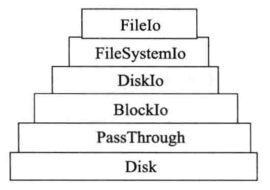
\includegraphics[width=10cm]{filesystem_protocol_stack.png}
    % 中文标题 %
    \caption*{图 2-5 统一可扩展固件接口文件系统协议栈}
    % 调整图片英文标题与下文距离 %
    \setlength{\belowcaptionskip}{-0.7cm}
    % 英文标题 %
    \caption*{Figure 2-5 UEFI File system protocol stack}
\end{figure}

如图2-5所示,最下层Disk层表示如硬盘设备这样的块设备硬件。PassTh-\newline rough层表示硬盘设备与总线接口的协议,
EFI\_ATA\_PASS\_THRU\_PROTOCOL提供有关ATA控制器以及将ATA命令块发送到与该ATA控制器相连的任何ATA设备的信息。
而EXT\_SCSI\_PASS\_THRU\_PROTOCOL协议提供了将ATAPI命令块发送到连接到该ATA控制器或SCSI控制器的ATAPI设备
的功能。此协议可直接操作硬盘具体扇区中的数据内容,为UEFI内核提供最底层的硬盘接口功能函数。
\par 再往上一层是块输入输出BlockIo(下同)层,BlockIo是可扩展固件接口输入输出协议EFI\_BLOCK\_IO\_PROTOCOL
的缩写,主要提供了按块访问设备的功能,包括块的读写函数和刷新flush函数。再往上一层的硬盘输入输出DiskIo层,
在BlockIo的基础上进行再次封装,DiskIo为EFI\_DISK\_IO\_PROTOCOL的缩写。此协议提供了从磁盘任
意地址读写任意长度数据的功能,这也符合了硬盘作为块设备可以随机访问数据的特点。
\par 再往上一层为文件系统输入输出FileSystemIo(下同)层,他对应于简易文件系统协议EFI\_SIMPLE\_FILE\_SYSTEM
\_PROTOCOL协议,这个协议是对文件系统驱动加载时,驻留在内存中的文件系统功能函数的引用和封装。再往上一层为文件
输入输出FileIo层,对应于EFI\_FILE\_PROTOCOL协议,用于对以文件为单位的数据进行操作。在UEFI运行环境中如Shell环
境中加载.efi文件时,就经历了从下到上完整的协议栈的过程,最终以文件数据流的形式传递给Shell环境,并完成后续的执
行或其他加载操作。

\subsection{相关驱动介绍}
UEFI中的驱动大致分为两类:一类是符合UEFI驱动模型的驱动,成为“UEFI驱动”;另一类是不遵循UEFI驱动模型的驱动,
称为“DXE驱动”,也称为服务型驱动。服务型驱动加载过程较为简单,在Image初始化的时候,即在执行模块入口函数时,
将Protocol安装到自身Handle即可。
如2.1节中UEFI协议运作方式的介绍可知,UEFI协议作为一个包含了所需功能函数指针的结构体,需要具体的UEFI驱动程序
为其实现所需的功能。
UEFI文件系统协议栈相关的驱动程序分别为:AtaatapiPassThruDxe、PartitionDxe、DiskIoDxe、FileSysDxe,
从命名可以看出,他们四个驱动都属于DXE驱动即服务型驱动,用于在UEFI的DXE和BDS阶段为系统提供服务,其中
的PassThruDxe和FileSysDxe根据具体的硬盘接口与具体文件系统不同而定。其中PassThruDxe驱动程序负责定义硬盘设备
与ATA或SCSI总线进行数据交互的功能;PartitionDxe用于解析存储在硬盘ESP分区中的GPT分区表,用于获取到硬盘中数据
的分区信息,磁盘在使用前都要进行分区,也就是将硬盘划分为一个个逻辑的区域,不同的分区上可装载不同的文件系统,以
方便用户使用。
GPT分区表示意图如图2-6所示。GPT(GUID Partition Table):全局唯一标识磁盘分区表\cite{extra3},是一个实体硬盘的
分区表的结构布局的标准,是可扩展固件接口(EFI)标准,被用于替代BIOS系统中的一64bits来存储逻辑块地址和大小信
息的主开机纪录(MBR)分区表,与普遍使用的主引导记录(MBR)分区方案相比,GPT提供了更加灵活的磁盘分区机制。
LBA(Logical Block Addressing)逻辑块寻址模式将CHS这种三维寻址方式转变为一维的线性寻址,它把硬盘所有
物理扇区的C/H/S编号通过一定的规则转变为一线性的编号,系统效率得到大大提高,避免了烦琐的磁头/柱面/扇区
的寻址方式。如图中的LBA0扇区为保护MBR,它的作用是阻止不能识别GPT分区的磁盘工具试图对其进行分区或格式化
等操作。LBA1扇区开始则为分区表和表项,每个表项对应一个用户区域内的磁盘分区,并表识这个分区的开始和结束
位置。关于GPT分区表的详细分析及恶意篡改方式将在第三章中介绍。

\begin{figure}[htb]
    %\label{ffs_format}
    % 调整图片与上文的垂直距离 %
    \vspace{0cm}   
    % 调整图片图片与中文标题、中文标题与英文标题距离 %
    \setlength{\abovecaptionskip}{0.3cm}  
    % 引用/fig/目录中的图片文件 %
	\centering
    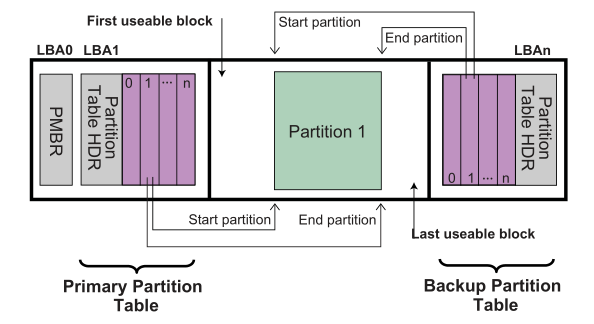
\includegraphics[width=10cm]{partition.png}
    % 中文标题 %
    \caption*{图 2-6 硬盘全局分区表示意图}
    % 调整图片英文标题与下文距离(本文标准为-0.7cm) %
    \setlength{\belowcaptionskip}{-0.7cm}
    % 英文标题 %
    \caption*{Figure 2-6 Hard disk GPT partition}
\end{figure}

DiskIoDxe驱动用于定义硬盘最基础的输入输出数据功能,也就是等同于操作系统中的硬盘驱动程序;而
FileSysDxe驱动则负责为UEFI提供与硬盘硬件相同的文件系统数据组织形式,用以在UEFI系统中通过UNIX风格的文件系统
为其他模块提供硬盘文件的交互功能支持。
%
% 2.4节
%
\section{BMC技术介绍}
BMC(Baseboard Management Controller)基板管理控制器是一种用于实时检测服务器硬件信息并具备独立运算能力的
计算机系统中的组件,它通过IPMI协议与服务器中的其他硬件设备进行通信。在基于IPMI协议的管理平
台中,系统对平台各个硬件设备的信息管理策略,都是通过与BMC通信并统计运算而实现
的\cite{addition5,addition6}。BMC拥有除了独立处理器外的独立固件闪存、系统电源、网卡设备,是一个具有独立性的基于服务器平台的管理
子系统。在如今的服务器国产化过程中,BMC越来越得到各个厂商的广泛使用。

\subsection{BMC与BIOS通讯方式}
IPMI协议作为BMC与服务器其他硬件设备通信的桥梁主要有两种通信方式,他们分别是BT(Block Transfer)接口
和KCS(Keyboard Controller Style)接口,其中BT接口主要是用于传输数据的块传输,即最小传输单位设置为一块,
256字节。而KCS接口主要用于以最小单位为一字节来进行数据传输。而在BIOS与BMC的通信过程中,主要使用BMC来
进行一些度量过程中基准值的存储功能,因此使用KCS接口来进行通讯设计,以避免不必要的传输资源浪费。

\begin{figure}[htb]
    %\label{ffs_format}
    % 调整图片与上文的垂直距离 %
    \vspace{0cm}   
    % 调整图片图片与中文标题、中文标题与英文标题距离 %
    \setlength{\abovecaptionskip}{0.3cm}  
    % 引用/fig/目录中的图片文件 %
	\centering
    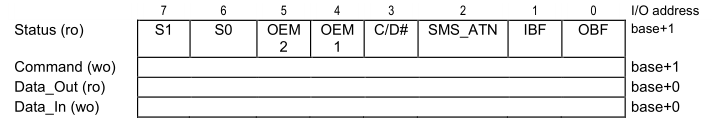
\includegraphics[width=12cm]{kcs_register.png}
    % 中文标题 %
    \caption*{图 2-7 KCS接口寄存器信息}
    % 调整图片英文标题与下文距离(本文标准为-0.7cm) %
    \setlength{\belowcaptionskip}{-0.7cm}
    % 英文标题 %
    \caption*{Figure 2-7 KCS Interface Registers}
\end{figure}

如图2-7所示,为KCS接口所使用到的寄存器即相关信息,主要涉及到四个寄存器,分别是用来查看BMC此时状态的状态
寄存器、用于指定BMC命令的命令寄存器、和两个分别用来进行数据输入和数据输出缓存的寄存器。有关这些寄存器具体
使用方法和使用流程将在第四章的BMC驱动实现中做详细说明。

%
% 2.5节
%
%\section{可信计算技术}

%\subsection{可信计算信任链}

%\subsection{可信平台模块}

%
% 2.5节
%
\section{本章小结}
本章首先介绍了UEFI规范中的整体系统设计结构,并着重介绍了UEFI的协议运作方式和对本文有重要作用的启动时服务
提供的具体功能函数。然后对固件文件系统中驱动数据的存放方式进行了描述,为后面的驱动内容读取功能提供了理论基础;
分析了UEFI文件系统协议栈在系统中的作用和具体到主要的四个驱动程序名称。最后对UEFI BIOS中与BMC系统的通信方式
进行了分析,选用了IPMI的KCS访问模式,来完成数据的交互。

\bjutclearpage
%
% 第三章
%
\chapter{基于UEFI的硬盘文件安全加载策略研究}
\label{cha:architecture}

%
% 3.1节
%
\section{安全漏洞分析}
UEFI环境中,加载硬盘设备上的ESP分区中的系统文件是一个十分丰富的过程,它不仅包含了UEFI系统内部的文件加载
过程,它还包含着如硬盘分区的创建、硬盘文件系统的建立、操作系统安装过程中向ESP分区内添加操作系统引导文件
BootLoader等文件的过程,以及UEFI环境中识别硬盘分区方式、识别硬盘特定分区中的文件系统并通过UEFI内部
的相同文件系统格式定义,使其完成UEFI内核与硬盘设备间的文件数据交互功能\cite{chinese19}。
\par 本节将介绍硬盘文件系统的建立过程,UEFI环境中硬盘文件加载的过程,以及从硬盘硬件层面和从UEFI固件层面
两方面对硬盘文件进行攻击以达到篡改ESP分区中关键系统文件的可能性。
\subsection{硬盘文件系统建立过程分析}
在一个服务器或个人电脑上安装操作系统时,其实都经历着硬盘文件系统建立的过程\cite{chinese22}。如图3-1所示,
中建立GPT硬盘
分区格式的目的为让UEFI可识别出硬盘分区的信息,传统MBR分区格式只能由传统BIOS系统识别。为硬盘创建FAT文件
系统的目的也在于统一硬件上的数据组织形式和UEFI内存中的硬盘数据处理格式\cite{extra1}。

\begin{figure}[htb]
    \label{ffs_format}
    % 调整图片与上文的垂直距离 %
    \vspace{0cm}   
    % 调整图片图片与中文标题、中文标题与英文标题距离 %
    \setlength{\abovecaptionskip}{0.3cm}  
    % 引用/fig/目录中的图片文件 %
	\centering
    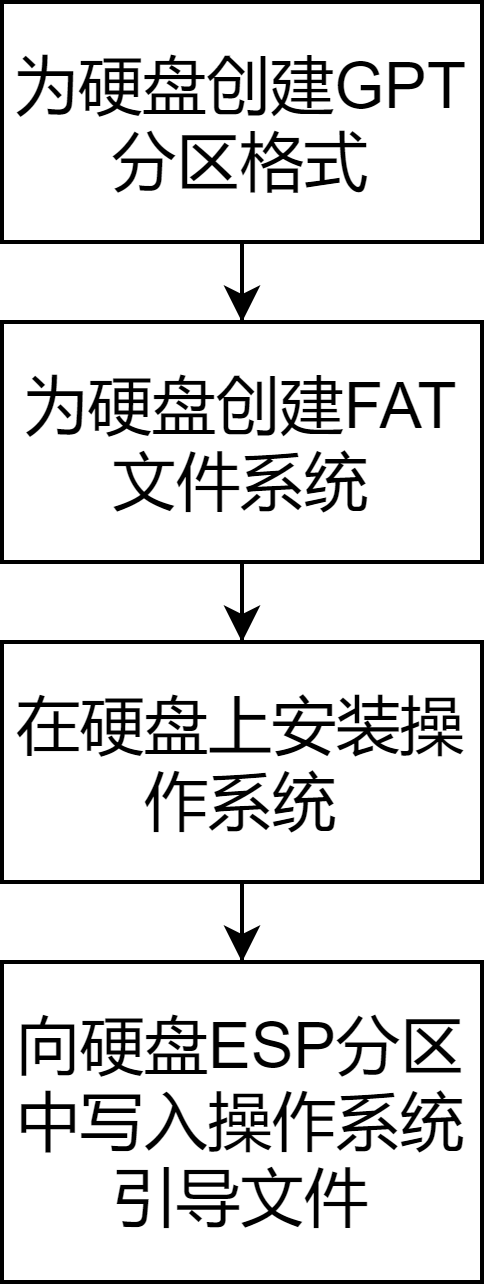
\includegraphics[width=2cm]{disk_init.png}
    % 中文标题 %
    \caption*{图 3-1 硬盘文件系统建立过程}
    % 调整图片英文标题与下文距离(本文标准为-0.7cm) %
    \setlength{\belowcaptionskip}{-0.7cm}
    % 英文标题 %
    \caption*{Figure 3-1 Hard disk file system establishment process}
\end{figure}

而ESP分区之所以作为EFI系统分区,是因为在安装操作系统的过程中,操作系统安装程序将GPT分区格式硬盘
的其中一个分区初始化为ESP分区,并将引导加载操作系统其他模块的BootLoader引导程序等系统关键EFI程序,
放入到这个自己建立的ESP分区中。这样便有了UEFI环境中加载硬盘设备ESP分区中系统引导文件及其他关键EFI
文件的由来。

\subsubsection{服务器启动流程分析}
UEFI BIOS作为一个基础输入输出系统,为操作系统提供基础的硬件支持,同时也能引导操作体统的启动,具体
实施方式为:

\begin{figure}[htb]
    \label{ffs_format}
    % 调整图片与上文的垂直距离 %
    \vspace{0cm}   
    % 调整图片图片与中文标题、中文标题与英文标题距离 %
    \setlength{\abovecaptionskip}{0.3cm}  
    % 引用/fig/目录中的图片文件 %
	\centering
    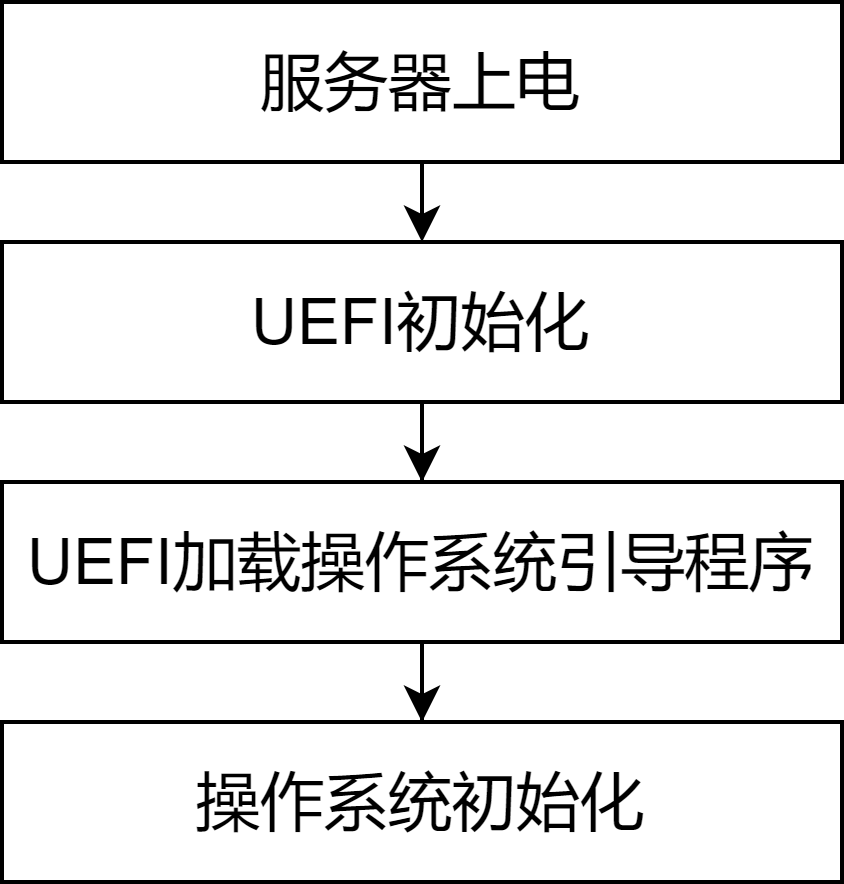
\includegraphics[width=4cm]{server_start.png}
    % 中文标题 %
    \caption*{图 3-2 服务器启动流程}
    % 调整图片英文标题与下文距离(本文标准为-0.7cm) %
    \setlength{\belowcaptionskip}{-0.7cm}
    % 英文标题 %
    \caption*{Figure 3-2 Server startup process}
\end{figure}

如图3-2所示,服务器上电,随后初始化UEFI BIOS系统,再由UEFI系统通过内部的文件系统协议栈加载硬盘ESP
分区中的操作系统引导文件,随后控制权交给引导程序并退出UEFI系统初始化流程。本文重点研究的过程是UEFI
初始化过程,和UEFI加载硬盘ESP分区文件过程。
如图3-3所示,为UEFI系统的初始化流程。

\begin{figure}[htb]
    \label{ffs_format}
    % 调整图片与上文的垂直距离 %
    \vspace{0cm}   
    % 调整图片图片与中文标题、中文标题与英文标题距离 %
    \setlength{\abovecaptionskip}{0.3cm}  
    % 引用/fig/目录中的图片文件 %
	\centering
    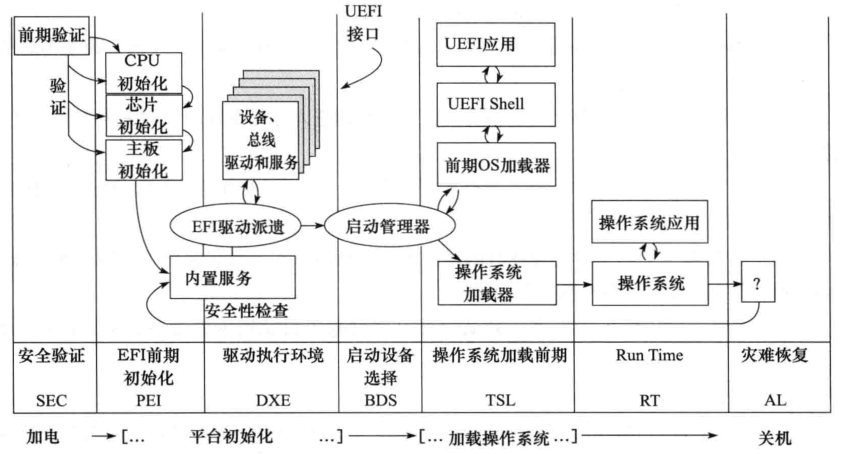
\includegraphics[width=12cm]{uefi_boot_process.png}
    % 中文标题 %
    \caption*{图 3-3 UEFI启动流程}
    % 调整图片英文标题与下文距离(本文标准为-0.7cm) %
    \setlength{\belowcaptionskip}{-0.7cm}
    % 英文标题 %
    \caption*{Figure 3-3 UEFI boot process}
\end{figure}

如图所示,UEFI系统在遵循UEFI标准的SEC安全启动阶段后,进入PEI和DXE两个UEFI初始化阶段关键的驱动程序加载
过程,在这里完成UEFI系统的内存及内存地址的建立、硬件设备驱动程序的加载、硬件设备存储器I/O端口映射等系统
关键初始化步骤。随后通过BDS阶段的BDS core核心程序,也就是启动管理器程序,加载位于硬盘ESP分区中的前期
OS加载器以及操作系统加载器。其中,前期OS加载器用来作为SHELL用户接入程序、PXE网络启动程序等这些过程的
引导器使用;而操作系统加载器则负责引导服务器上在UEFI启动前安装的特定操作系统。

\subsection{UEFI环境文件加载过程分析}
由前面的分析可知,UEFI环境中的硬盘文件加载过程建立在硬盘块设备已经建立好GPT分区格式和与UEFI内核中对应
的文件系统格式的前提下,通过UEFI文件系统协议栈的层级关系,一层一层调用来实现硬盘文件数据加载到UEFI系统
内存的过程。

\begin{figure}[htb]
    \label{ffs_format}
    % 调整图片与上文的垂直距离 %
    \vspace{0cm}   
    % 调整图片图片与中文标题、中文标题与英文标题距离 %
    \setlength{\abovecaptionskip}{0.3cm}  
    % 引用/fig/目录中的图片文件 %
	\centering
    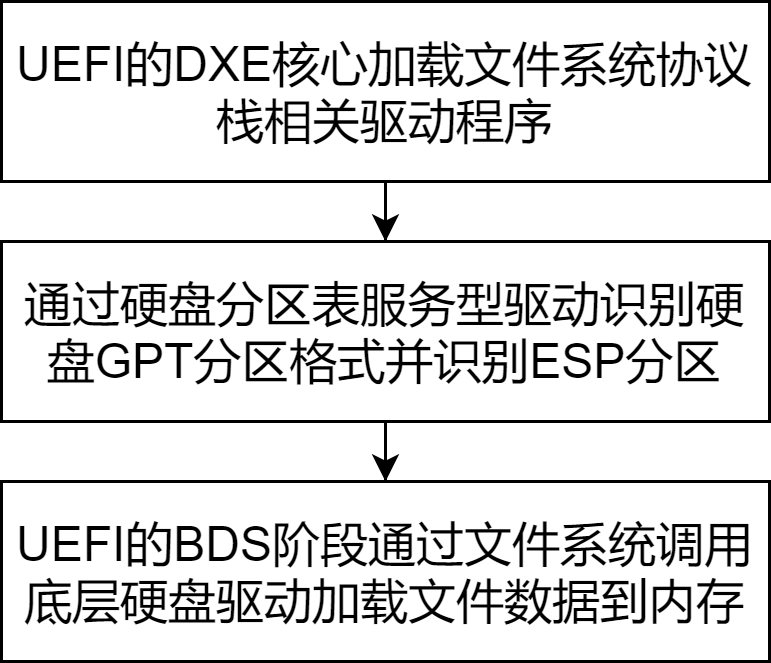
\includegraphics[width=6cm]{uefi_loadfile_process.png}
    % 中文标题 %
    \caption*{图 3-4 UEFI文件加载过程}
    % 调整图片英文标题与下文距离(本文标准为-0.7cm) %
    \setlength{\belowcaptionskip}{-0.7cm}
    % 英文标题 %
    \caption*{Figure 3-4 UEFI load file process}
\end{figure}

如图3-4所示,UEFI会先通过DXE加载UEFI文件系统协议栈相关的驱动程序,具体驱动程序为:PassThruDxe、
PartitionDxe、DiskIoDxe、FileSysDxe四个驱动,其中PassThruDxe和FileSysDxe会根据具体系统的不同
而确定不同的特定硬盘接口和文件系统。通过加载UEFI文件系统协议栈驱动程序,UEFI内核已经完成了文件系统
协议栈的建立,包括各个驱动功能函数在UEFI永久内存中的驻留以及对应UEFI协议对特定硬盘驱动的函数引用;
再通过在DXE阶段加载的PartitionDxe硬盘分区表服务型驱动程序,识别出硬盘的GPT分区格式并获取到GPT分区
表,通过GPT分区表再得到硬盘的ESP分区的起始和结束扇区位置,从而确定UEFI内核在BDS阶段读取操作系统
引导文件的分区位置;接下来就是UEFI进入BDS阶段并通过文件系统协议栈加载硬盘ESP分区中的文件到内存中,
并移交控制权到这个EFI可运行文件身上。
\par UEFI文件系统协议栈加载硬盘文件数据的过程,从函数调用的角度看,就是上层FileIo系统调用,调用
通过FileSysDxe加载得到的UEFI内核中的文件系统,并通过文件系统调用底层的由PassThruDxe和DiskIoDxe
驱动提供的硬盘驱动程序。在UEFI环境中,驱动功能的调用通过与其对应并对其引用的协议完成。

\subsection{从硬盘攻击关键文件}
有了对前面的硬盘分区和文件系统,UEFI系统内的文件系统的建立过程和UEFI环境中文件的加载过程的了解,
可知黑客可通过硬件手段攻击位于硬盘硬件设备上的文件系统结构\cite{chinese33}、和攻击用来存储BIOS的固件芯片两方面,
来到达篡改UEFI加载硬盘文件的文件内容。

\begin{figure}[htb]
    \label{ffs_format}
    % 调整图片与上文的垂直距离 %
    \vspace{0cm}   
    % 调整图片图片与中文标题、中文标题与英文标题距离 %
    \setlength{\abovecaptionskip}{0.3cm}  
    % 引用/fig/目录中的图片文件 %
	\centering
    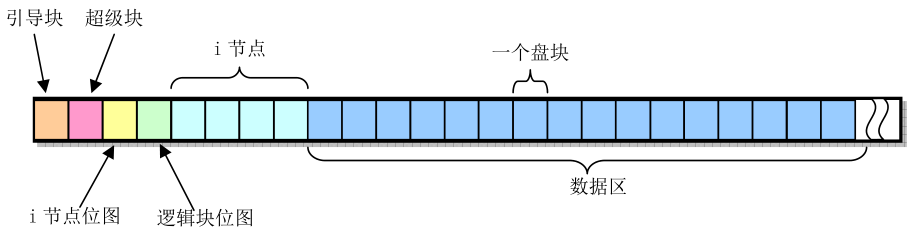
\includegraphics[width=13cm]{minix_fs_layout.png}
    % 中文标题 %
    \caption*{图 3-5 MINIX文件系统硬盘布局}
    % 调整图片英文标题与下文距离(本文标准为-0.7cm) %
    \setlength{\belowcaptionskip}{-0.7cm}
    % 英文标题 %
    \caption*{Figure 3-5 MINIX file system hard disk layout}
\end{figure}

\par 首先是针对硬盘设备的攻击,如图3-5所示,是MINIX文件系统在硬盘上的数据结构布局图\cite{chinese30},
作为一个类
UNIX文件系统,其与标准UNIX文件系统的设计结构基本相同,FAT文件系统和ext2文件系统也同样属于类UNIX
文件系统。由于各种类UNIX文件系统的基础设计理念和结构基本相同,不同之处仅在于更新一代的文件系统会
提供更为丰富的如数据恢复、文件操作日志记录等内容,而底层基础功能结构不变,因此以MINIX作为说明\cite{chinese31}。
\par 其中引导块对应于UEFI系统中硬盘的ESP分区,里面装载了操作系统所需的引导程序。超级块用于存放
盘设备上文件系统结构的信息,并说明各个部分大小。i节点位图用于说明i节点是否被使用,每个比特位代表
一个i节点。逻辑块位图用于描述盘上的每个数据盘块的使用情况,每个比特位代表盘上数据区中的一个盘块。
盘上的i节点部分存放着文件系统中文件或目录的索引节点,每个文件或目录都对应一个i节点。其中每个特定
文件对应的i节点数据结构中,都存有一个其包含的所有文件数据磁盘块的映射关系,用于通过i节点索引文件
数据。
\par 由以上分析可知,黑客可通过技术手段将恶意代码文件事先存入硬盘ESP分区或引导块中\cite{chinese32},
并获取到恶意
代码文件和UEFI将加载的系统文件分别对应的i节点,然后通过硬件手段修改i节点数据结构中文件数据块映射
的关系,将系统文件链接到恶意代码文件的数据块链,使UEFI加载系统文件时实际运行的却是恶意代码。因此
在UEFI系统中,在加载硬盘系统文件或关键文件前,对其进行完整性测量以保证加载的文件没有经过篡改,这
个过程就显得十分必要。

\subsection{从固件芯片攻击关键驱动}
作为UEFI内核与硬盘硬件设备连接的桥梁,文件系统定义了双方共同的数据组织形式和结构,来达到数据互通
的效果。因此,作为存储在BIOS固件系统上的文件系统驱动程序,同样可以作为黑客用来篡改硬盘ESP分区中
关键文件信息的攻击对象。

\begin{figure}[htb]
    \label{ffs_format}
    % 调整图片与上文的垂直距离 %
    \vspace{0cm}   
    % 调整图片图片与中文标题、中文标题与英文标题距离 %
    \setlength{\abovecaptionskip}{0.3cm}  
    % 引用/fig/目录中的图片文件 %
	\centering
    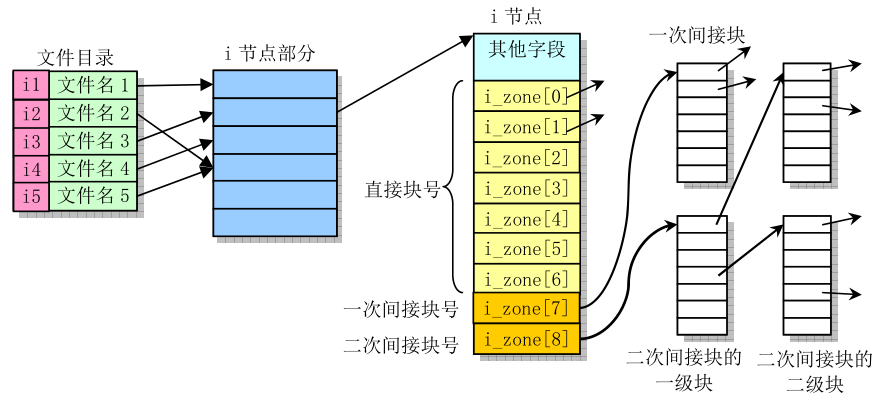
\includegraphics[width=13cm]{fs_inode_zone.png}
    % 中文标题 %
    \caption*{图 3-6 内存中的文件系统索引文件方式}
    % 调整图片英文标题与下文距离(本文标准为-0.7cm) %
    \setlength{\belowcaptionskip}{-0.7cm}
    % 英文标题 %
    \caption*{Figure 3-6 Method of index file by file system in memory}
\end{figure}

如图3-6所示,当UEFI加载了文件系统驱动之后,内存中便驻留了文件系统组织文件的方式及特定的数据结构。
当UEFI系统通过文件名索引硬盘中的文件数据时,会通过目录项这个数据结构中的i节点信息确定这个绝对路径下
特定文件名对应的硬盘中的i节点,并以此来获取到文件数据。
\par 在这个文件系统内部通过文件名检索文件数据的过程中,黑客可以通过改变文件目录项中文件名与i节点
的对应关系,来篡改特定系统文件名所对应的具体硬盘数据内容\cite{chinese15}。同样可以在内存的文件系统中,
更改i节点与
文件数据块关系,也就是更改图3-6中的i\_zone指针所指向的位置,来完成恶意代码数据对系统文件数据的更替
效果。因此,在UEFI加载文件系统模块及其相关驱动前,对他们在BIOS固件芯片中内容进行完整性度量,以确保
UEFI运行的是可信的文件系统代码,可以从固件层面消除黑客对硬盘文件内容篡改的可能。

%
% 3.2节
%
\section{信任链的设计}
在对UEFI文件系统协议栈驱动程序和硬盘ESP分区中系统关键EFI文件进行可信度量的同时,需要首先建立UEFI
系统的可信启动。根据TCG平台规范,本文选用具有存储UEFI驱动程序度量基准值功能的BMC系统作为UEFI可信
启动信任链的可信平台模块\cite{chinese5},用包含基准值存取、可信度量日志记录基本功能的BMC来作为替代传统TPM的底层
平台\cite{chinese25}。

\begin{figure}[htb]
    \label{ffs_format}
    % 调整图片与上文的垂直距离 %
    \vspace{0cm}   
    % 调整图片图片与中文标题、中文标题与英文标题距离 %
    \setlength{\abovecaptionskip}{0.3cm}
    % 引用/fig/目录中的图片文件 %
	\centering
    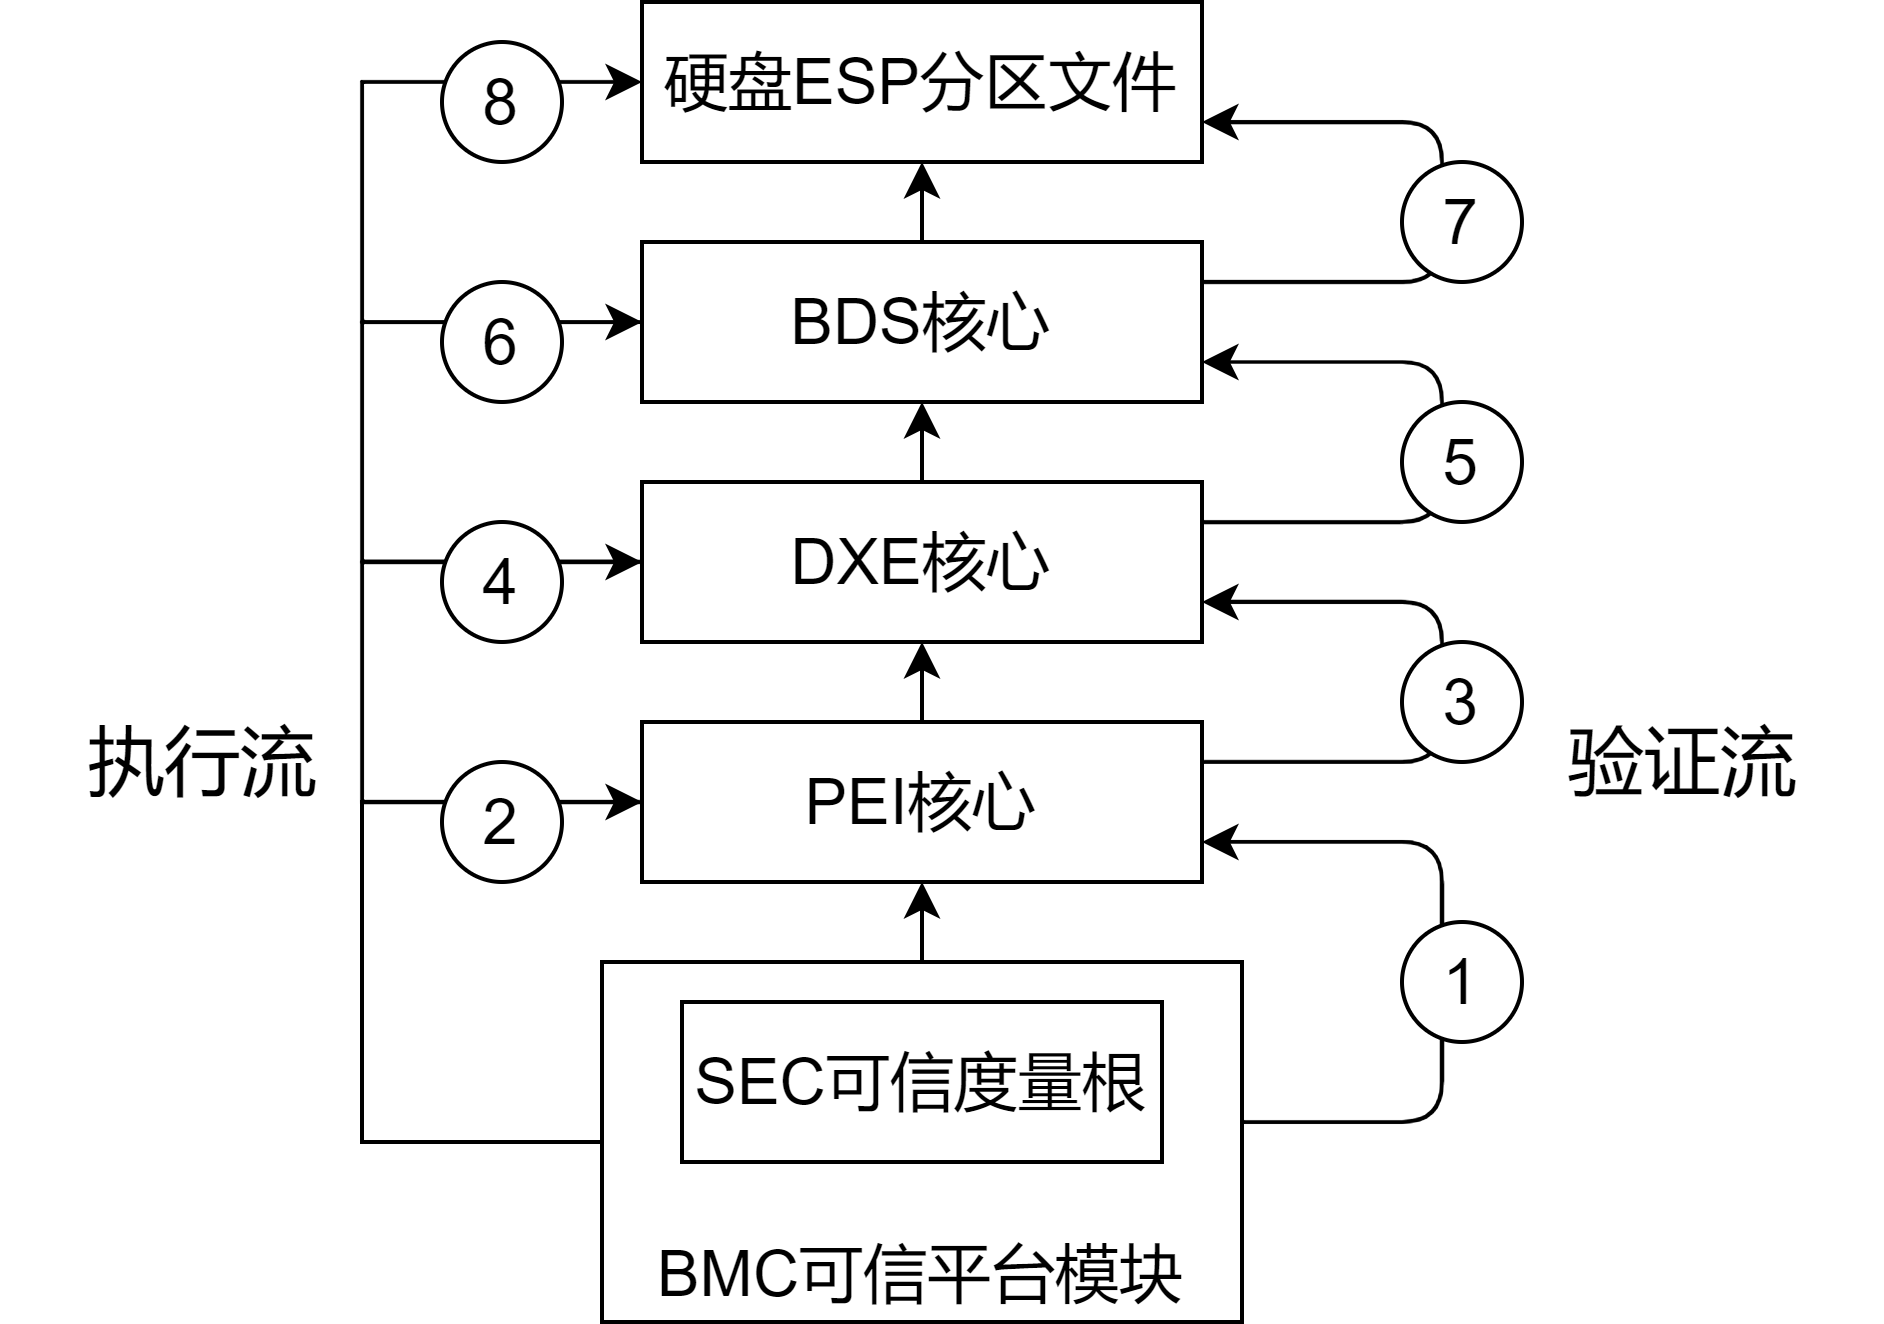
\includegraphics[width=10cm]{trust_link.png}
    % 中文标题 %
    \caption*{图 3-7 UEFI信任链传递}
    % 调整图片英文标题与下文距离(本文标准为-0.7cm) %
    \setlength{\belowcaptionskip}{-0.7cm}
    % 英文标题 %
    \caption*{Figure 3-7 UEFI trusted chain transfer}
\end{figure}

如图3-7所示,信任链以BMC系统作为可信平台模块\cite{chinese27,chinese28},并以UEFI的第一阶段SEC启动
阶段作为信任链中的可信根\cite{chinese6}。
然后在SEC阶段,借助BMC系统中的可信平台模块对PEI阶段的核心代码进行可信度量,在得到可信度量的结果
为PEI核心可信时,将系统控制权交给PEI核心;PEI核心借助BMC中的基准值,对系统cpu、主板和芯片组的PEIM
组件进行可信度量,并根据度量结果最后对DXE核心进行度量,并将系统控制权交给DXE核心;DXE核心阶段加载
系统其余组件,同时对UEFI文件系统协议栈的驱动程序进行度量,以保证在BDS阶段加载硬盘文件时,数据流所
经过的底层UEFI文件系统协议栈可信。最后对BDS核心进行可信度量;系统控制权交给BDS阶段核心代码,在
加载硬盘ESP分区中关键文件时,对文件内容进行度量,若可信,再将控制权交给文件进行UEFI系统调用\cite{chinese12}。

%
% 3.3节
%
\section{安全方案设计}
根据UEFI启动阶段信任链的设计,本安全方案涉及到的UEFI启动阶段为SEC、PEI、DXE、BDS,以做到在保证
硬盘文件数据经过的硬盘设备、硬盘文件系统协议栈安全可信的同时,还要保证在BDS阶段加载硬盘文件时,
BDS核心代码的安全可信。因此安全方案分成SEC、PEI、DXE、BDS四个阶段进行设计\cite{english1},下面将对安全方案在
各个阶段的设计进行描述。

\subsection{SEC阶段}
SEC(Security Phase)阶段是UEFI平台初始话的第一个阶段,计算机系统加电后首先进入这个阶段。SEC阶段
首先接收并处理系统启动和重启信号,系统加电信号、系统重启信号、系统运行过程中的异常信号。还有一个重要
过程为初始化临时存储区域。系统运行在SEC阶段时,仅CPU和CPU内部资源被初始化,而各种外部设备和内存都没
有被初始化。因此系统需要一部分临时内存用于代码和数据的存储,一般称为临时RAM,临时RAM只能位于CPU内部
。最常用的临时RAM是Cache,把其当成内存使用,这种技术称为CAR(Cache As RAM)。
\par SEC阶段的目的是为PEI阶段准备一切所需的资源,包括了通过CAR得到的RAM地址和大小、栈地址和大小以及
固件卷fv的位置,使PEI可以通过这些信息加载系统资源及后续流程。本安全方案在SEC阶段的设计为,度量PEI 
core代码,得到度量结果,并判断是否将控制权由SEC传递给PEI。

\begin{figure}[htb]
    \label{ffs_format}
    % 调整图片与上文的垂直距离 %
    \vspace{0cm}   
    % 调整图片图片与中文标题、中文标题与英文标题距离 %
    \setlength{\abovecaptionskip}{0.3cm}
    % 引用/fig/目录中的图片文件 %
	\centering
    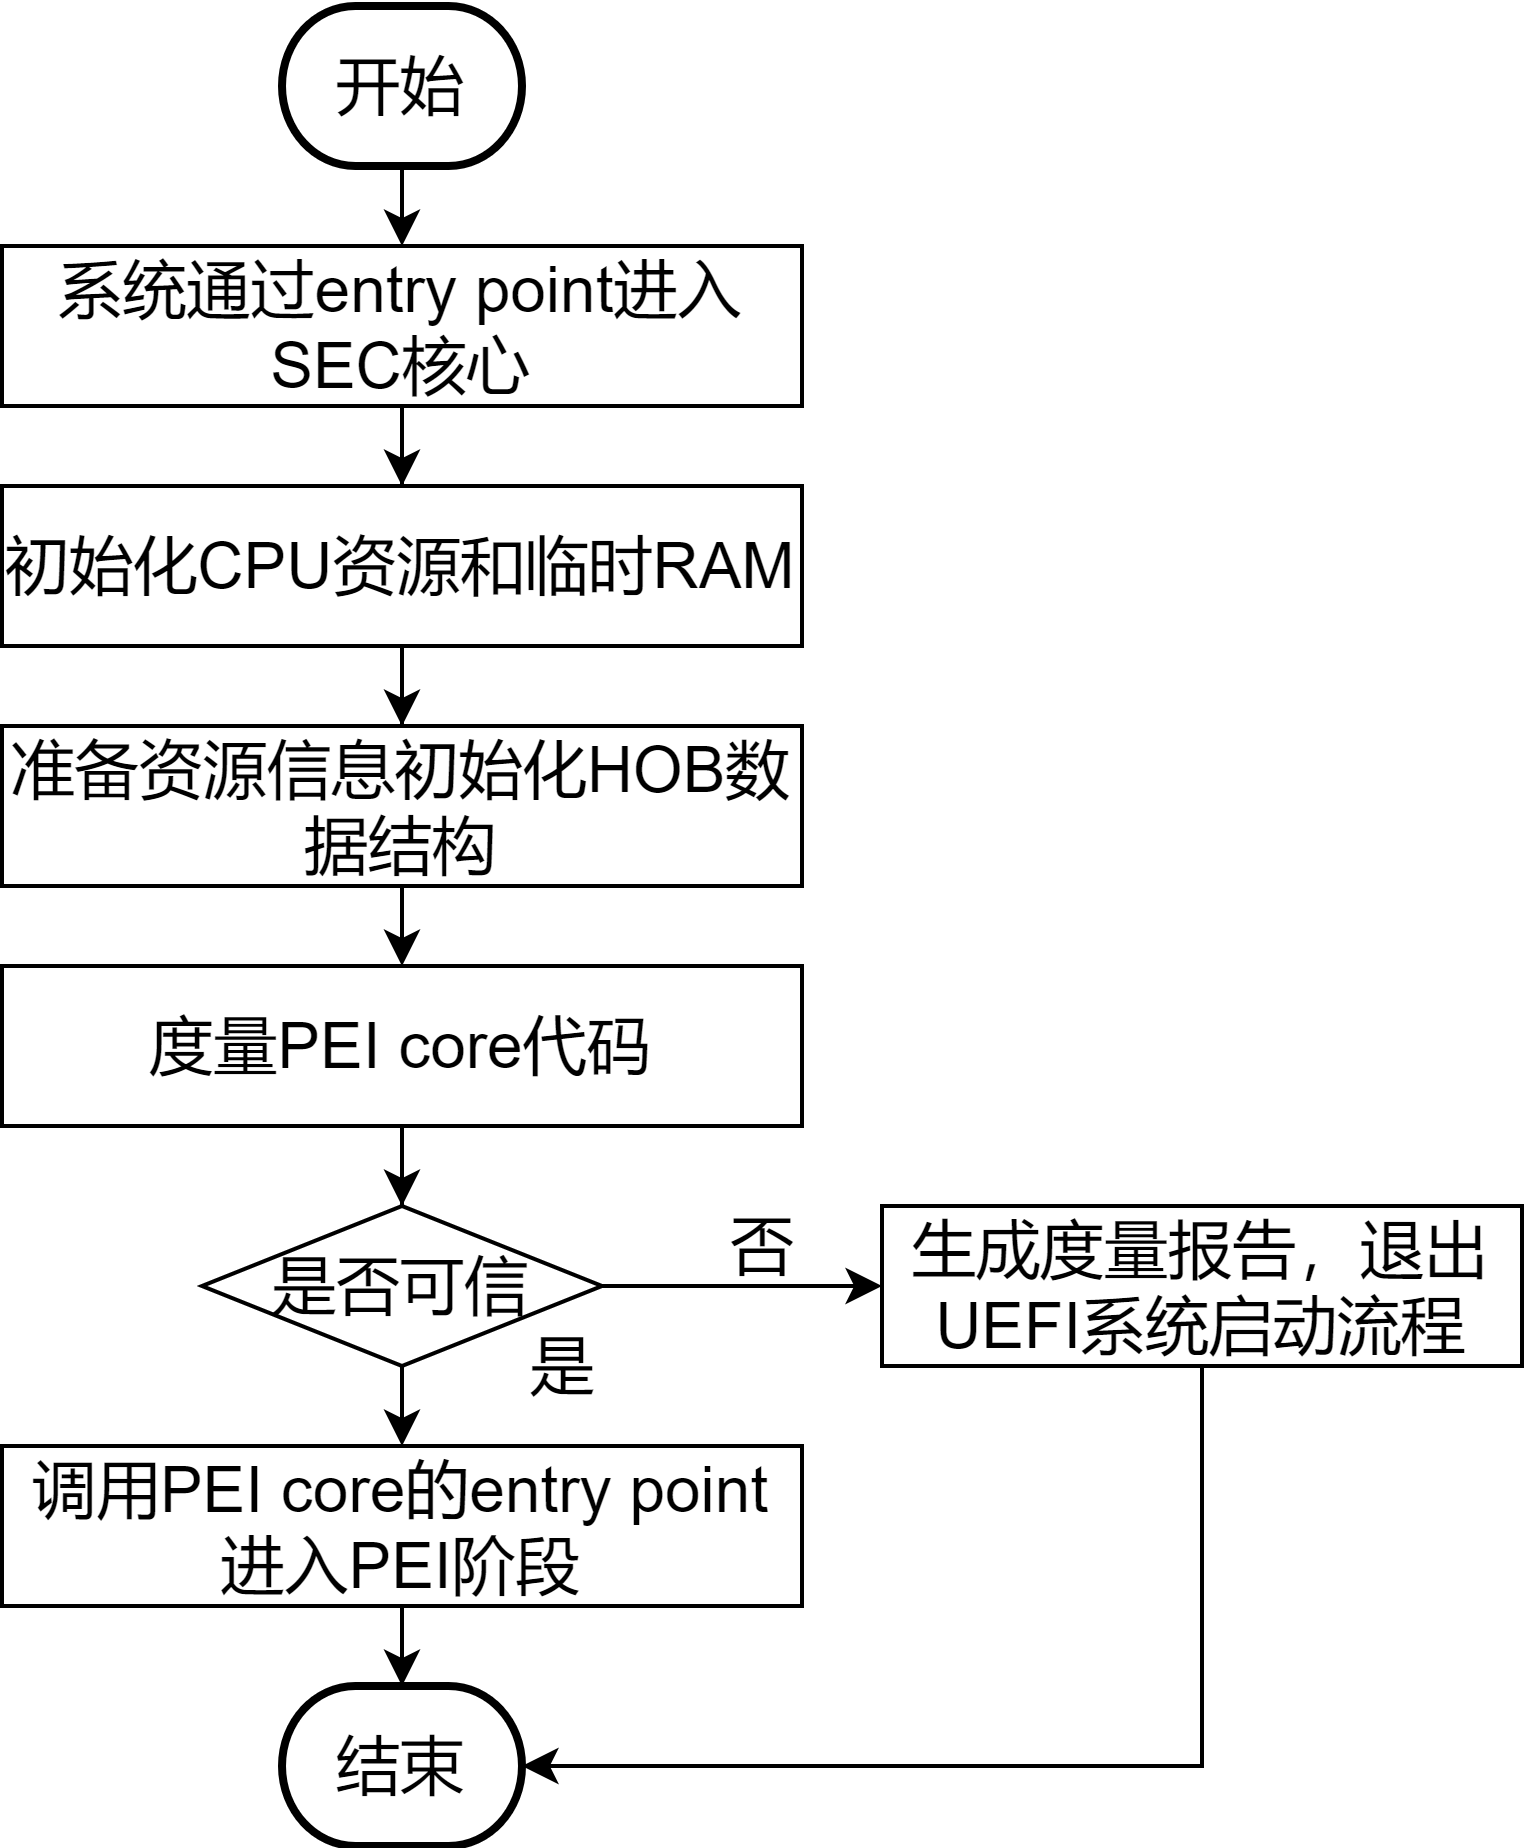
\includegraphics[width=8cm]{sec_process.png}
    % 中文标题 %
    \caption*{图 3-8 SEC阶段执行流程}
    % 调整图片英文标题与下文距离(本文标准为-0.7cm) %
    \setlength{\belowcaptionskip}{-0.7cm}
    % 英文标题 %
    \caption*{Figure 3-8 Execution process of SEC}
\end{figure}

如图3-8所示,在系统正常执行SEC阶段代码中加入可信度量PEI core代码的过程,并根据度量结果,若PEI core
内容可信,则控制权交给PEI的entry point入口函数,否则停止UEFI启动流程,并生成度量日志。

\subsection{PEI阶段}
系统控制权到了PEI(Pre-EFI Initialization)阶段,并由PEI core核心代码负责运行PEI阶段的功能。虽然SEC
阶段对CPU和CPU内的资源进行了初始化,但是PEI阶段可用的资源依旧十分有限,该阶段对内存进行初始化,主要功
能是为DXE阶段准备执行环境,将所需要传递给DXE的信息组成HOB(Hand Off Block)列表,最终将控制权转交到DXE。
\par PEI和DXE一个不同之处在于,DXE拥有适量的系统永久RAM可供使用;而PEI仅仅拥有一些有限的临时RAM,
并且这些临时RAM在PEI阶段初始化永久内存后可能会被重新配置以作其它的用途,比如缓存(Cache)。因此,
PEI没有DXE的资源丰富。而PEI阶段的一个主要目的就是以最少的系统资源初始化永久内存,也就是UEFI系统和后面
的操作系统都可以使用的系统全部内存空间。
\par FV(Firmware Volume)的内容遵循EFI闪存文件系统的格式。PEI基础按照EFI闪存文件系统的格式来
发现FV中的PEIM。一个平台特有的PEIM可以通知PEI基础系统中的其它固件卷所处的
位置,这就允许PEI基础在其它固件卷体中找到PEIM。PEI基础和PEIM在EFI闪存文件
系统中用一个唯一的ID来命名。

\begin{figure}[htb]
    \label{ffs_format}
    % 调整图片与上文的垂直距离 %
    \vspace{0cm}   
    % 调整图片图片与中文标题、中文标题与英文标题距离 %
    \setlength{\abovecaptionskip}{0.3cm}
    % 引用/fig/目录中的图片文件 %
	\centering
    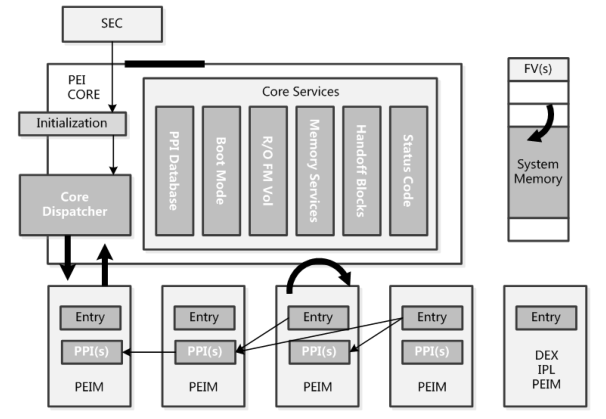
\includegraphics[width=12cm]{pei_core.png}
    % 中文标题 %
    \caption*{图 3-9 PEI阶段系统结构}
    % 调整图片英文标题与下文距离(本文标准为-0.7cm) %
    \setlength{\belowcaptionskip}{-0.7cm}
    % 英文标题 %
    \caption*{Figure 3-9 System structure of PEI}
\end{figure}

如图3-9所示,PEI阶段的主要结构分为PEI core也就是PEI基础代码,负责PEI阶段的整体功能执行;
PEI阶段的系统服务,用于PEI阶段功能函数的调用;PEI Dispatcher调度程序,用于调用FV固件卷中
的PEIM模块,其中就包括系统最基本的cpu、主板和芯片组的PEIM。当一个PEIM调度完成之后,PEI调
度程序将继续检查固件容卷,直到出现下列两种情况之一为止:
\par (1)所有被发现的PEIM都已经被调度
\par (2)不再有PEIM可被调度
\par 这是因为任何PEIM都不能满足上述列出的调度条件。一旦达到上述两个条件中的任一个,PEI调度
程序的工作就完成了,并且它调用一个用于启动下一阶段框架的架构PPI,即DXE初始程序加载
(Initial Program Load, IPL)PPI。

\begin{figure}[htb]
    \label{ffs_format}
    % 调整图片与上文的垂直距离 %
    \vspace{0cm}   
    % 调整图片图片与中文标题、中文标题与英文标题距离 %
    \setlength{\abovecaptionskip}{0.3cm}
    % 引用/fig/目录中的图片文件 %
	\centering
    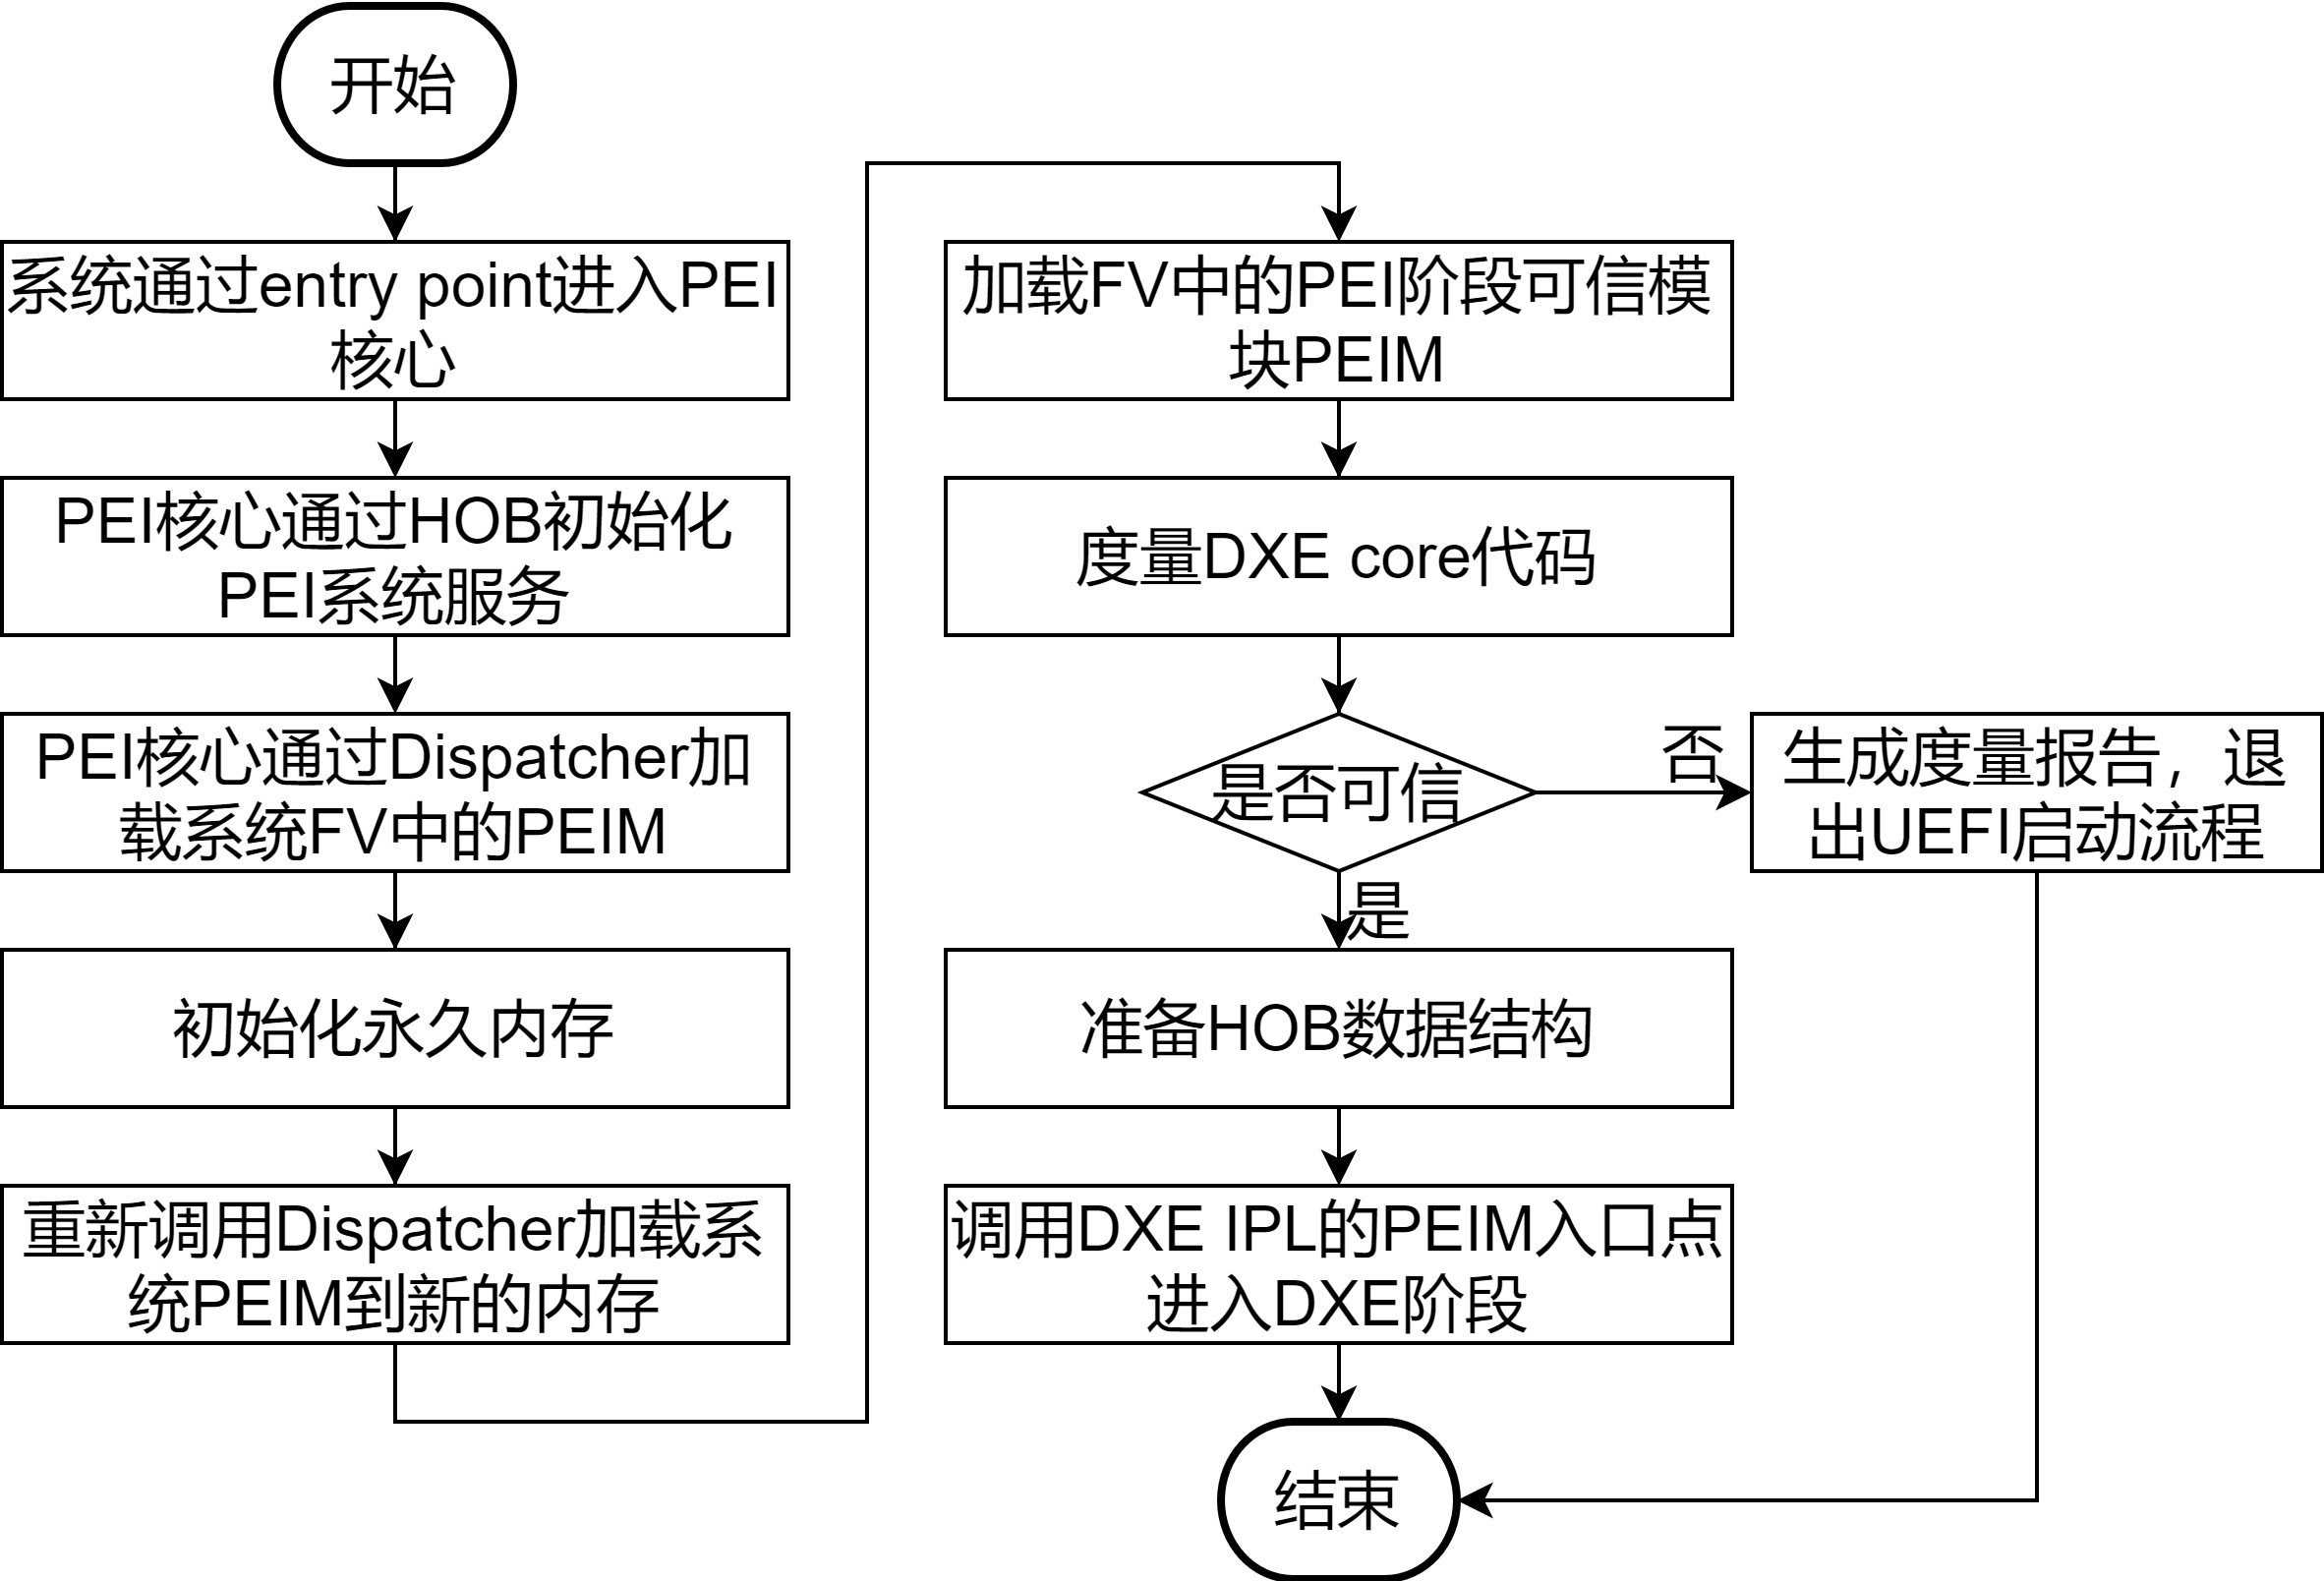
\includegraphics[width=12cm]{pei_process.png}
    % 中文标题 %
    \caption*{图 3-10 PEI阶段流程图}
    % 调整图片英文标题与下文距离(本文标准为-0.7cm) %
    \setlength{\belowcaptionskip}{-0.7cm}
    % 英文标题 %
    \caption*{Figure 3-10 Execution process of PEI}
\end{figure}

如图3-10所示,为本安全方案设计的PEI阶段流程。UEFI系统进入PEI阶段后,首先根据从SEC阶段传来
的HOB数据结构初始化PEI系统服务,用于给PEIM的加载过程提供支持;然后通过PEI阶段的调度程序加载
位于FV固件卷中的PEIM程序,除了cpu、主板和芯片组的PEIM外还包括如提供PPI通信协议的PEIM等内容;
随后PEI core通过这些最小的功能集合初始化UEFI系统的永久内存;在系统获得永久内存后,PEI core
再次调用PEIM调度程序,这次的目的是在完整的永久内存中加载这些PEIM,并在永久内存中执行后面流程;
随后加载FV中的PEI阶段的可信度量模块PEIM,用这个PEIM的功能度量FV中的DXE core代码,并根据度量
结果继续加载DXE core或是停止UEFI启动流程。

\subsection{DXE阶段}
DXE阶段为本安全方案度量UEFI文件系统协议栈驱动程序的主要系统启动阶段,目的是为后面BDS阶段通过
文件系统协议栈加载硬盘文件时,保证内核中文件系统服务程序的安全可靠。由于此安全方案的主要目的为
保证UEFI环境加载硬盘文件的安全可信,因此将DXE驱动度量范围缩小至UEFI文件系统协议栈相关驱动,
达到减小系统开销的目的。

\begin{figure}[htb]
    \label{ffs_format}
    % 调整图片与上文的垂直距离 %
    \vspace{0cm}   
    % 调整图片图片与中文标题、中文标题与英文标题距离 %
    \setlength{\abovecaptionskip}{0.3cm}
    % 引用/fig/目录中的图片文件 %
	\centering
    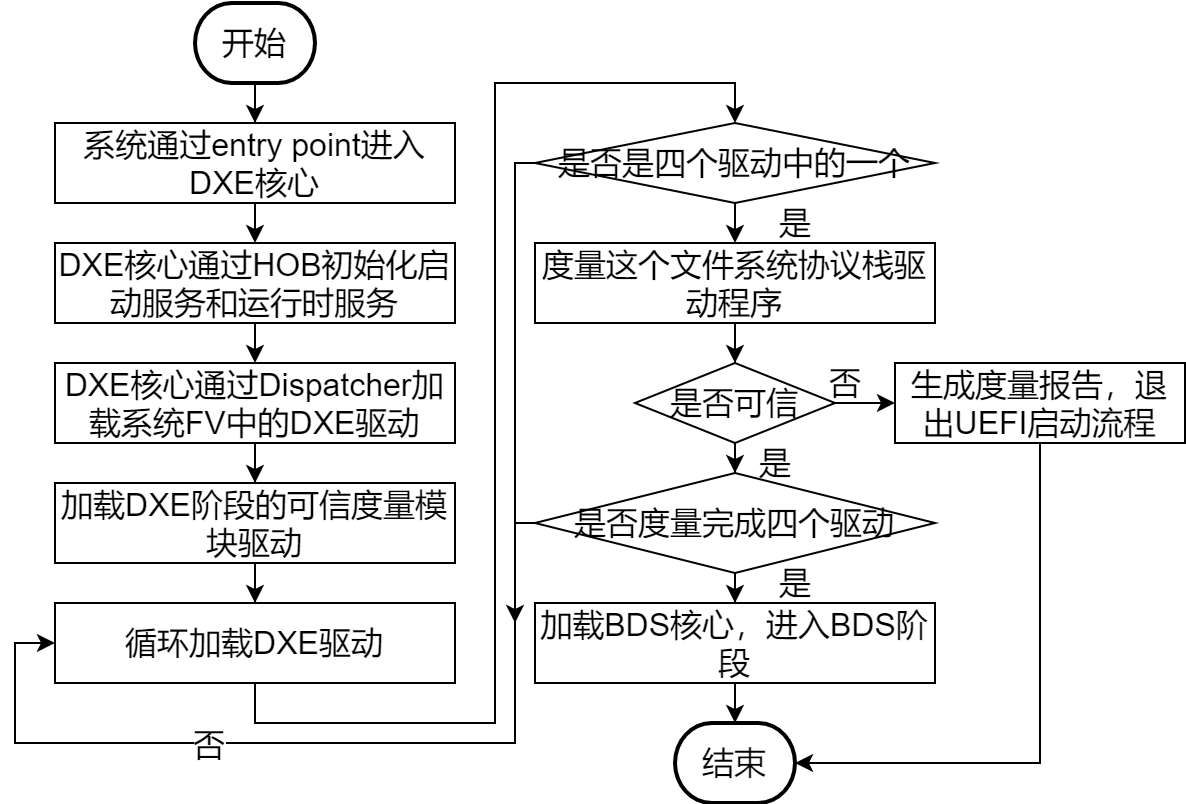
\includegraphics[width=12.3cm]{dxe_process.png}
    % 中文标题 %
    \caption*{图 3-11 DXE阶段流程图}
    % 调整图片英文标题与下文距离(本文标准为-0.7cm) %
    \setlength{\belowcaptionskip}{-0.7cm}
    % 英文标题 %
    \caption*{Figure 3-11 Execution process of DXE}
\end{figure}

如图3-11所示,系统进入DXE阶段后,首先根据PEI阶段传来的HOB数据结构初始化DXE阶段的Boot Service
和Runtime Service,用以给DXE阶段的驱动程序及其加载提供系统服务;随后控制权交给DXE阶段的调度
程序调度DXE驱动的加载,根据DXE驱动程序的依赖表达式,调度程序会首先加载那些系统相关度较低的驱动
程序,根据安全方案的设计,需要在加载UEFI文件系统协议栈的四个相关的驱动之前加载DXE阶段的可信度量
驱动。由于PEI和DXE两个阶段使用不同的系统服务,而可信度量模块中需要分别使用到PEI系统服务和DXE系统
服务,因此为PEI和DXE阶段分别设计两个可信度量功能的相关模块或驱动;之后在加载四个文件系统协议栈的
驱动程序前分别对其进行可信度量;根据四个驱动的可信度量结果,若都可信,则继续加载后续驱动并将系统
控制权最终交给BDS core,否则,停止UEFI系统启动。

\subsection{BDS阶段}
BDS core通过BDS架构协议定位和加载在启动准备服务环境中执行的各种各样的应用。这些应用可
能表示一个传统的OS启动装载程序,或者表示可代替最终的OS运行或在加载最终的OS之前运行的扩展服务。
这样的扩展启动准备服务可能包括安装配置、扩展诊断、闪存更新支持、OEM服务,或者OS启动代码。

\begin{figure}[htb]
    \label{ffs_format}
    % 调整图片与上文的垂直距离 %
    \vspace{0cm}   
    % 调整图片图片与中文标题、中文标题与英文标题距离 %
    \setlength{\abovecaptionskip}{0.3cm}
    % 引用/fig/目录中的图片文件 %
	\centering
    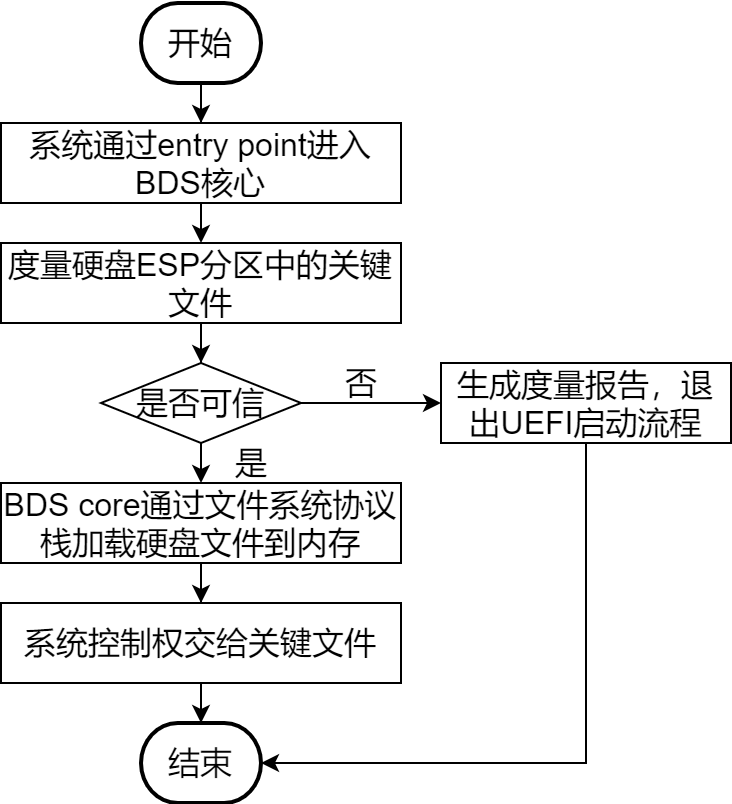
\includegraphics[width=8cm]{bds_process.png}
    % 中文标题 %
    \caption*{图 3-12 BDS阶段流程图}
    % 调整图片英文标题与下文距离(本文标准为-0.7cm) %
    \setlength{\belowcaptionskip}{-0.7cm}
    % 英文标题 %
    \caption*{Figure 3-12 Execution process of BDS}
\end{figure}

如图3-12所示,系统进入BDS阶段执行BDS core代码,并根据BDS加载的硬盘ESP分区中的文件调用DXE阶段
加载的可信度量服务型驱动对该文件进行可信度量,若结果可信,则通过UEFI文件系统协议栈加载此文件
到UEFI系统的永久内存中,并交给此文件系统的控制权;否则停止该文件的加载,退出UEFI启动。

%
% 3.4节
%
\section{固件驱动与硬盘文件度量设计}
根据前面所述的安全方案的UEFI启动各个阶段的度量设计,可看出此安全方案的重点在于DXE阶段对UEFI文件
系统协议栈驱动程序的度量,以及BDS阶段对硬盘ESP分区中关键文件的度量工作。图3-13展示了此安全方案在
DXE阶段的总体功能设计。

\begin{figure}[htb]
    \label{ffs_format}
    % 调整图片与上文的垂直距离 %
    \vspace{0cm}   
    % 调整图片图片与中文标题、中文标题与英文标题距离 %
    \setlength{\abovecaptionskip}{0.3cm}
    % 引用/fig/目录中的图片文件 %
	\centering
    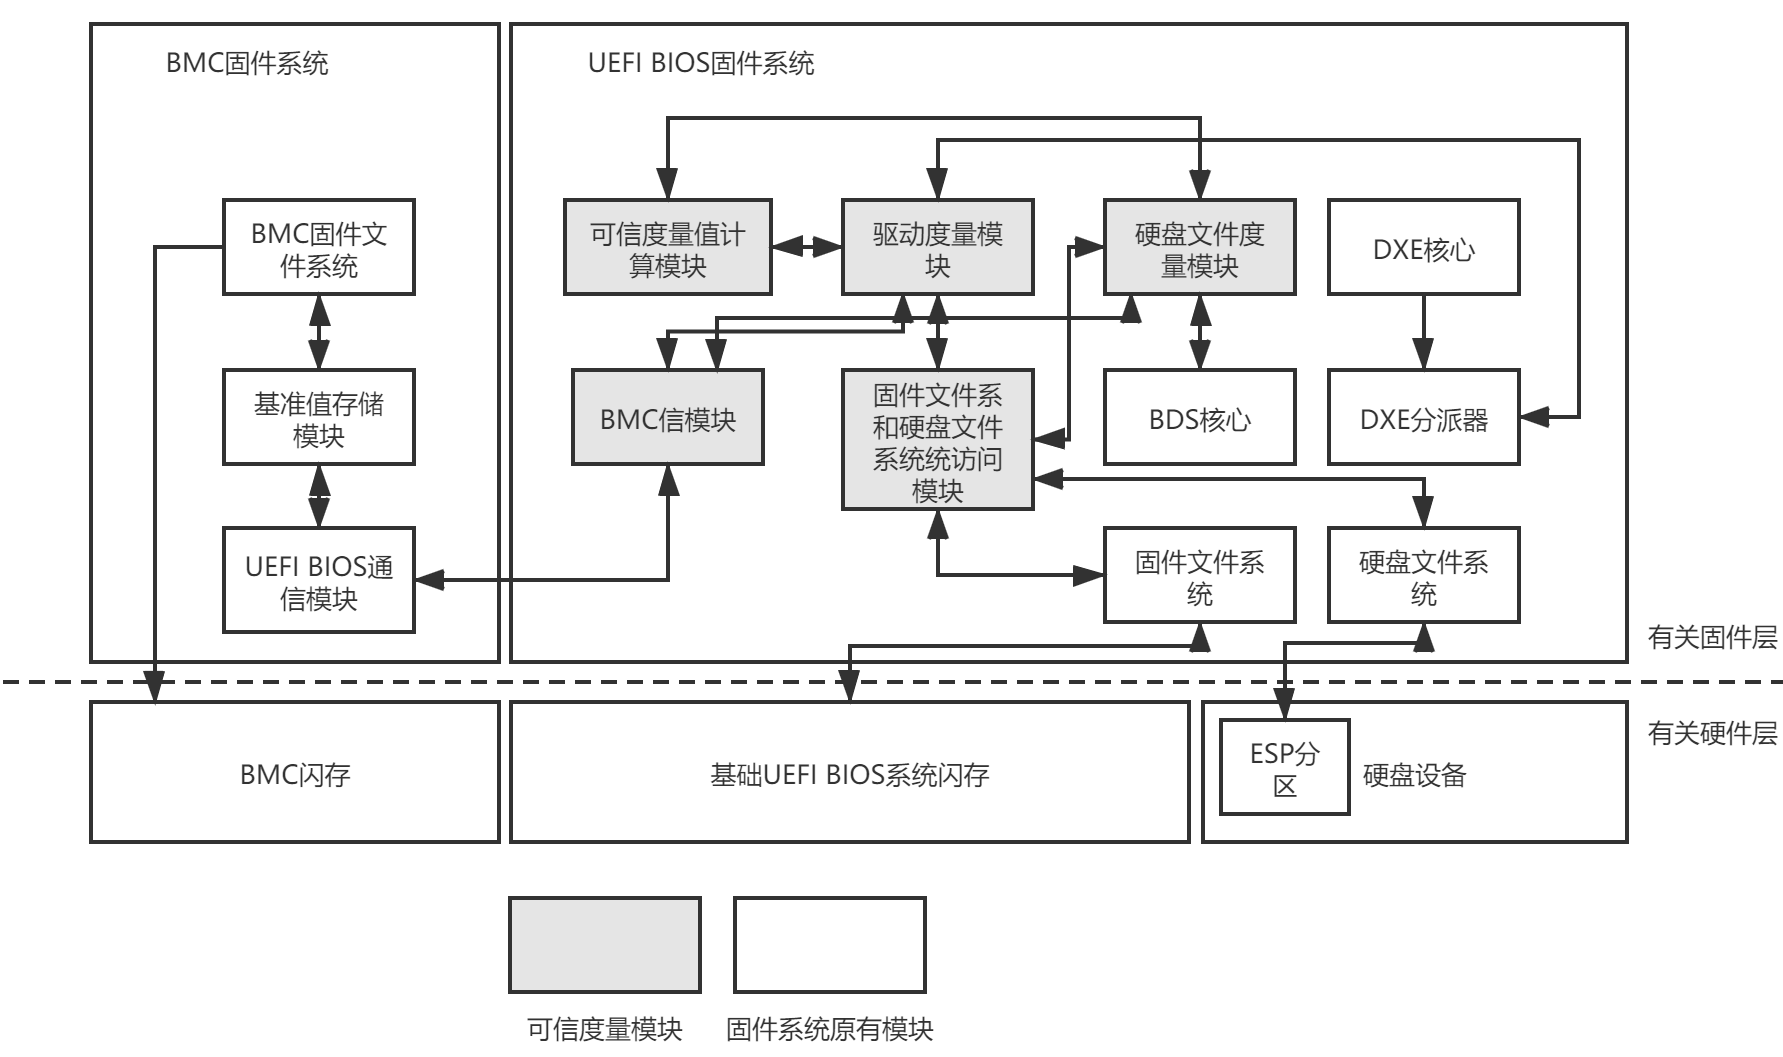
\includegraphics[width=14cm]{system_framework.png}
    % 中文标题 %
    \caption*{图 3-13 系统结构图}
    % 调整图片英文标题与下文距离(本文标准为-0.7cm) %
    \setlength{\belowcaptionskip}{-0.7cm}
    % 英文标题 %
    \caption*{Figure 3-13 System framework}
\end{figure}

如图3-13所示,此系统涉及到用来存储各个阶段核心程序和文件系统协议驱动程序的基准值的BMC固件系统,而
此安全方案中的可信度量模块以DXE驱动程序的形式,存储于UEFI BIOS固件芯片中,并通过UEFI系统原有的
DXE core和DXE调度程序加载可信度量驱动至内存中。
\par 在度量过程中,由DXE阶段的调度程序给可信度量驱动中的驱动度量模块发送度量信号,由驱动度量模块
通过文件系统协议栈驱动的全局唯一标识信息匹配出四个驱动程序,并通过UEFI中的固件文件系统FFS获取到存储
于FV固件芯片中的驱动程序数据到UEFI内存,并调用可信度量值计算模块计算出FV中驱动的hash值;再调用BMC
通信模块,通过GUID获取到存储于BMC芯片中的度量基准值,通过驱动度量模块对基准值和度量值的比较得到度量
结果。
\par 到了BDS阶段,在BDS core加载硬盘文件前,通过调用硬盘文件度量模块负责调度其他可信度量模块,具体
过程和驱动度量模块相同,不同之处在于,所获得的硬盘数据文件需要通过UEFI文件系统协议栈加载存储于硬盘
ESP分区中的关键文件,并进行度量获得度量结果。

%
% 3.5节
%
\section{本章小结}
本章首先对UEFI系统加载硬盘ESP分区中文件数据的过程进行了分析,通过对文件系统数据组织结构的分析找出
了文件加载过程中的安全漏洞,并针对通过UEFI文件系统协议栈加载硬盘数据的过程,划分了UEFI启动不同阶段
中的安全方案,并提出了DXE阶段和BDS阶段所涉及到的可信度量驱动和相关模块的调用关系及BMC系统存储基准值
的作用,为后文安全方案的具体实施奠定了基础。

\bjutclearpage

%
% 第四章
%
\chapter{基于UEFI的硬盘文件可信加载详细设计}
\label{cha:detail_design}
%
% 4.1节
%
\section{度量计算模块设计}
%
% 4.2节
%
\section{硬盘文件度量模块设计}
%
% 4.3节
%
\section{驱动文件度量模块}
%
% 4.4节
%
\section{固件和硬盘访问模块设计}

\subsection{固件访问设计}

\subsection{硬盘访问设计}
%
% 4.5节
%
\section{BMC通信模块设计}

\subsection{BMC驱动设计}

\subsection{BMC驱动度量方式}
%
% 4.5节
%
\section{本章小结}



%
% 第五章
%
\chapter{硬盘文件安全加载方案测试及分析}
\label{cha:test}
有了三四章节的理论和代码基础,本章将在此基础上,逐步进行实验验证分析。验证内容包括,DXE阶段驱动程序度量功能
的验证、BDS阶段硬盘文件度量功能的验证、UEFI系统中BMC驱动程序的连通性验证、通过EDKII编译生成的fd固件文件格式
的验证以及DXE阶段修改驱动程序加载顺序的验证。下面将先对实验环境进行介绍,以及选用的原因。

%
% 5.1节
%
\section{实验环境}

\subsection{申威6A服务器真机环境}
实验的真机环境是可信固件实验室提供的申威6A型服务器,实验环境包括了固件的编译环境以及服务器中BMC提供的fd固件
文件烧写环境,具体信息如下:
\par (1)固件编译系统环境:Ubuntu 10.04版本,并配置uuid-dev-2.17包
\par (2)固件编译工具:原版gcc4.4.3,和申威定制的swgcc-4.5.3-交叉编译器
\par (3)EDKII信息:带有申威定制包SenweiPkg的EDKIIR13995版本
\par (4)BMC烧写环境:Ubuntu 16.04版本和Firefox浏览器
\par Ubuntu 10.04版本的选择主要原因在于它提供的C语言库函数版本问题,由于swgcc-4.5.3-交叉编译器的特殊性,
需要特定库版本的支持,在以往实验中这一点经过验证。由于真机环境上运行的固件是经过申威ALPHA64架构处理器指令集定
制的,因此根据编译环境的特殊性做一些编译方法的介绍。交叉编译器的设置是通过linux系统软链接的方式实现的:

\begin{lstlisting}
ln -s sw_64sw2-unknown-linux-gnu-ar swar
ln -s sw_64sw2-unknown-linux-gnu-as swas
ln -s sw_64sw2-unknown-linux-gnu-gcc swgcc
ln -s sw_64sw2-unknown-linux-gnu-ld swld
ln -s sw_64sw2-unknown-linux-gnu-objcopy swobjcopy    
\end{lstlisting}

通过以上命令分别将申威定制版本的gcc编译器链接到官方版本gcc的调用名称上面,来实现编译命令的调用。

\begin{figure}[htb]
    \label{ffs_format}
    % 调整图片与上文的垂直距离 %
    \vspace{0cm}   
    % 调整图片图片与中文标题、中文标题与英文标题距离 %
    \setlength{\abovecaptionskip}{0.3cm}
    % 引用/fig/目录中的图片文件 %
	\centering
    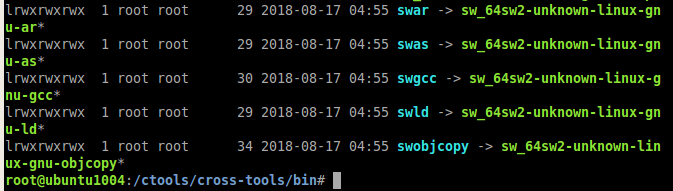
\includegraphics[width=12cm]{cross_tools.png}
    % 中文标题 %
    \caption*{图 5-1 编译器软连接}
    % 调整图片英文标题与下文距离(本文标准为-0.7cm) %
    \setlength{\belowcaptionskip}{-0.7cm}
    % 英文标题 %
    \caption*{Figure 5-1 Compiler Soft Link}
\end{figure}

图5-1所示的是查看软链接的修改效果。接下来是交叉编译申威固件程序的过程,首先需要使用原版gcc4.4.3编译器进行
edksetup程序的初始化工作,这个程序的目的在于为正在打开着的终端窗口设置好通过build编译时一切所需的环境变量
及一些通过C语言根据UEFI规范自动生成的代码内容。

\begin{figure}[htb]
    \label{ffs_format}
    % 调整图片与上文的垂直距离 %
    \vspace{0cm}   
    % 调整图片图片与中文标题、中文标题与英文标题距离 %
    \setlength{\abovecaptionskip}{0.3cm}
    % 引用/fig/目录中的图片文件 %
	\centering
    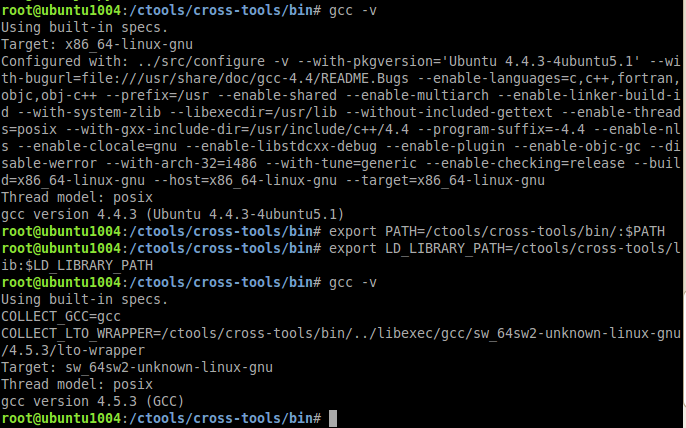
\includegraphics[width=12cm]{swgcc.png}
    % 中文标题 %
    \caption*{图 5-2 GCC版本切换过程}
    % 调整图片英文标题与下文距离(本文标准为-0.7cm) %
    \setlength{\belowcaptionskip}{-0.7cm}
    % 英文标题 %
    \caption*{Figure 5-2 GCC version switching process}
\end{figure}

如图5-2所示,是通过export改变环境变量的命令,将我们设置好的swgcc交叉编译器软链接目录添加到两个系统环境
变量中的过程,通过这样的方式,就可以实现用gcc 4.4.3版本进行edksetup程序的运行,并用swgcc交叉编译器进行
平台dsc文件的构建编译过程。具体编译过程,采用linux SHELL脚本的方式进行使用,如图5-3。

\begin{figure}[H]
    \label{ffs_format}
    % 调整图片与上文的垂直距离 %
    \vspace{0cm}   
    % 调整图片图片与中文标题、中文标题与英文标题距离 %
    \setlength{\abovecaptionskip}{0.3cm}
    % 引用/fig/目录中的图片文件 %
	\centering
    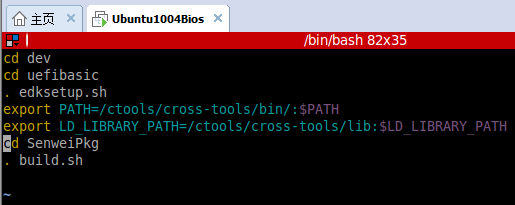
\includegraphics[width=12cm]{sw_sh_file.png}
    % 中文标题 %
    \caption*{图 5-3 交叉编译功能的终端程序}
    % 调整图片英文标题与下文距离(本文标准为-0.7cm) %
    \setlength{\belowcaptionskip}{-0.7cm}
    % 英文标题 %
    \caption*{Figure 5-3 Cross compile shell program}
\end{figure}

\begin{figure}[htb]
    \label{ffs_format}
    % 调整图片与上文的垂直距离 %
    \vspace{0cm}   
    % 调整图片图片与中文标题、中文标题与英文标题距离 %
    \setlength{\abovecaptionskip}{0.3cm}
    % 引用/fig/目录中的图片文件 %
	\centering
    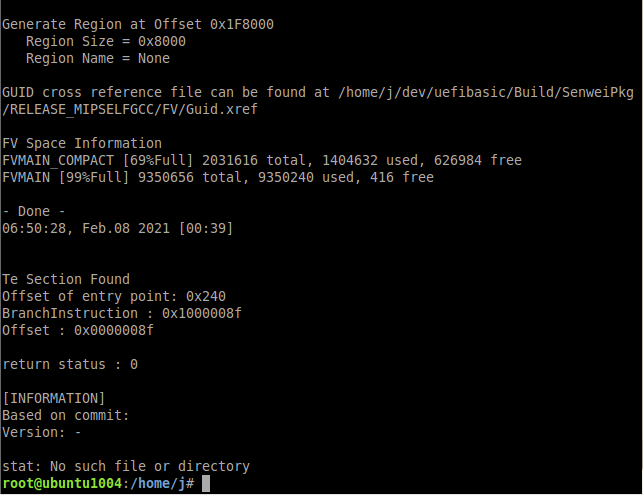
\includegraphics[width=12cm]{compile_res.png}
    % 中文标题 %
    \caption*{图 5-4 交叉编译结果}
    % 调整图片英文标题与下文距离(本文标准为-0.7cm) %
    \setlength{\belowcaptionskip}{-0.7cm}
    % 英文标题 %
    \caption*{Figure 5-4 Cross compile result}
\end{figure}

其中图5-3为开发的脚本语言编译程序,图5-4为最终的固件编译结果。

\subsection{UEFI Windwos模拟环境}
与真机环境对应的是Windows系统下的UEFI模拟运行环境,建立这个环境的目的在于,能够简化固件开发过程中调试的
复杂程度,通过模拟环境测试一些硬件结构不相关的功能模块运行效果,增加开发效率。其中具体信息如下:
\par (1)固件编译系统环境:Windows 10
\par (2)固件编译工具:VS2008
\par (3)EDKII信息:EDKIIR13995版本
\par 模拟环境的编译较为简单因此不做详细说明,编译效果图如图5-5。其中是GenFds命令生成最终fd固件文件的过程,
固件名称为NT32.fd。

\begin{figure}[htb]
    \label{ffs_format}
    % 调整图片与上文的垂直距离 %
    \vspace{0cm}   
    % 调整图片图片与中文标题、中文标题与英文标题距离 %
    \setlength{\abovecaptionskip}{0.3cm}
    % 引用/fig/目录中的图片文件 %
	\centering
    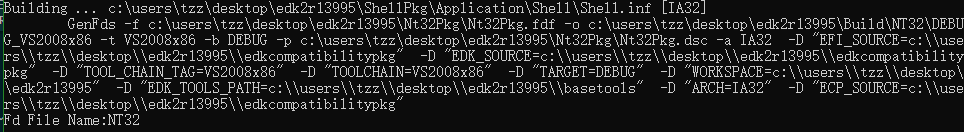
\includegraphics[width=12cm]{win_compile.png}
    % 中文标题 %
    \caption*{图 5-5 UEFI模拟环境编译结果}
    % 调整图片英文标题与下文距离(本文标准为-0.7cm) %
    \setlength{\belowcaptionskip}{-0.7cm}
    % 英文标题 %
    \caption*{Figure 5-5 UEFI simulation environment compilation results}
\end{figure}

%
% 5.2节
%
\section{驱动度量功能验证}
本文中在DXE阶段加载的可信度量驱动程序,主要用来度量四个UEFI文件系统协议栈驱动程序,并向BMC发送度量日志。
基于以上功能对可信度量驱动程序进行测试。

\subsection{测试目的}
该可信度量功能对DXE阶段特定驱动的度量方法存在普遍性,给出了根据现有UEFI驱动加载的设计理念,自定义度量驱动
内容的方法。该过程的正确性直接影响了BDS阶段加载硬盘文件的安全可信性。

\subsection{测试步骤}
(1)首先编写具有上述五个模块的DXE阶段可信度量驱动程序,并将其模块INF文件通过引用的方式添加到将要编译的申威平台
描述文件dsc文件中。
\par (2)然后通过本章第一节中的方法,对申威UEFI组件进行交叉编译。
\par (3)通过BMC芯片提供的网卡端口服务程序,用单独的客户端主机访问服务器上的网卡端口,此过程设置客户端
静态IP,设置成与BMC提供的服务IP同一网段内,并烧写UEFI BIOS固件文件到服务器的闪存芯片中。
\par (4)服务器上电并按电源按钮,进入UEFI BIOS启动流程,过程中将根据DXE阶段依赖,加载并度量四个特定驱动
程序。
\par (5)通过与步骤(3)同样的方法,通过网卡用客户端访问BMC,此时客户端需要安装default-jdk环境,并安装了
Maintance维护工具。通过lazyrrk 30 0命令获取BMC日志信息,其中包括驱动的度量日志。

\subsection{测试过程}
首先将经过交叉编译生成的SENWEI.fd文件通过BMC功能烧写如BIOS闪存中,如图5-6所示。将通过通过2400的控制器访问
并烧写提供的BIOS固件文件,烧写过程需要开机烧写,否则烧写失败\cite{chinese22}。

\begin{figure}[H]
    \label{ffs_format}
    % 调整图片与上文的垂直距离 %
    \vspace{0cm}   
    % 调整图片图片与中文标题、中文标题与英文标题距离 %
    \setlength{\abovecaptionskip}{0.3cm}
    % 引用/fig/目录中的图片文件 %
	\centering
    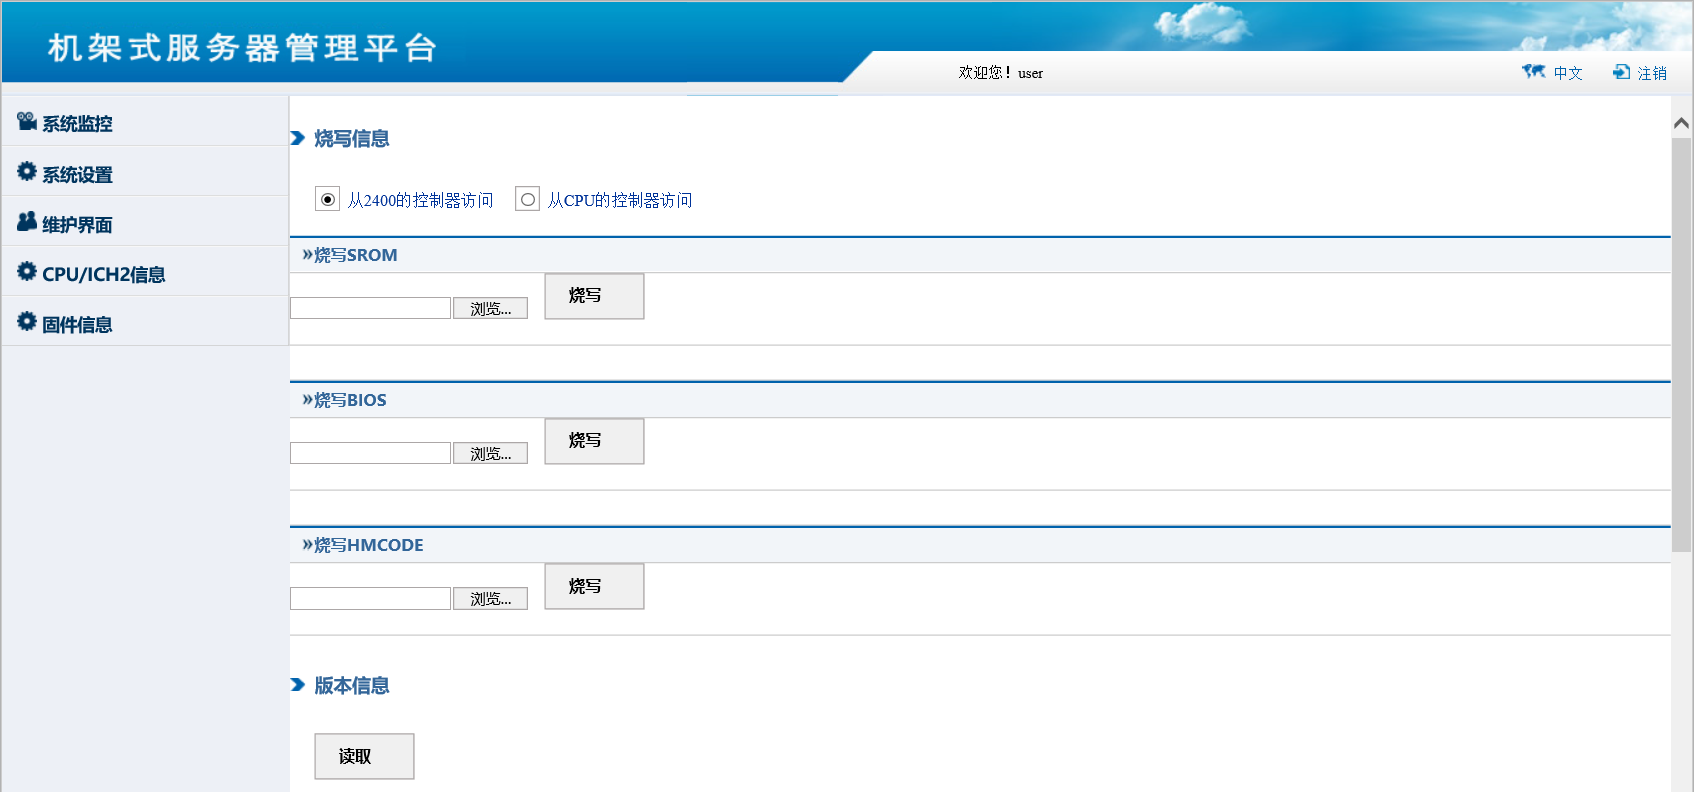
\includegraphics[width=12cm]{bmc.png}
    % 中文标题 %
    \caption*{图 5-6 BMC烧写固件界面}
    % 调整图片英文标题与下文距离(本文标准为-0.7cm) %
    \setlength{\belowcaptionskip}{-0.7cm}
    % 英文标题 %
    \caption*{Figure 5-6 BMC firmware interface}
\end{figure}

然后就是驱动度量日志的查看过程,通过安装的维护工具访问BMC特定端口,并通过linux系统中的重定向输出功能将读取
到的日志信息,写入指定的文件中。图5-7所示为四个特定驱动的度量日志。

\begin{figure}[H]
    \label{ffs_format}
    % 调整图片与上文的垂直距离 %
    \vspace{0cm}   
    % 调整图片图片与中文标题、中文标题与英文标题距离 %
    \setlength{\abovecaptionskip}{0.3cm}
    % 引用/fig/目录中的图片文件 %
	\centering
    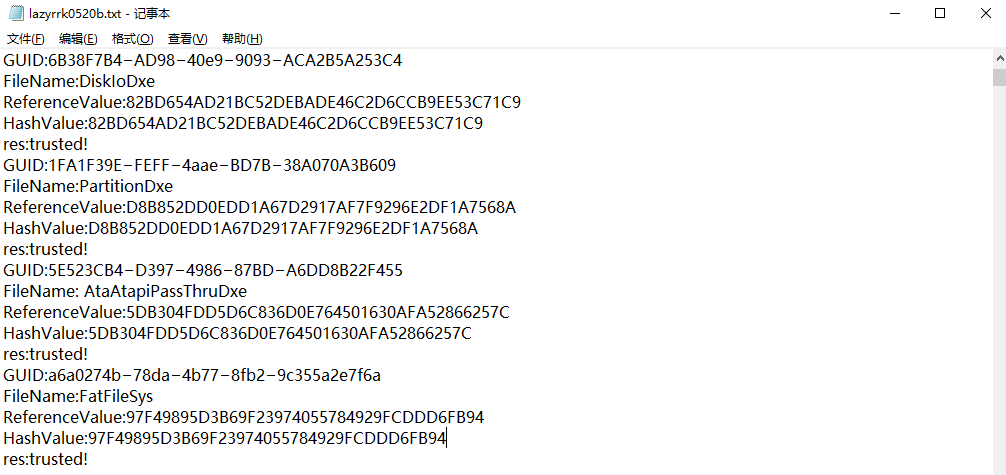
\includegraphics[width=12cm]{log.png}
    % 中文标题 %
    \caption*{图 5-6 驱动度量日志}
    % 调整图片英文标题与下文距离(本文标准为-0.7cm) %
    \setlength{\belowcaptionskip}{-0.7cm}
    % 英文标题 %
    \caption*{Figure 5-6 Driver mesurement log}
\end{figure}

%
% 5.3节
%
\section{BMC驱动连通性验证}

\subsection{测试目的}
在可信度量驱动程序的开发过程中,需要一个从BMC系统取出基准值的过程,通过单独测试UEFI BIOS中BMC驱动程序
的连通性有助于单独功能地调试可信度量驱动,保证BMC驱动的可用性。

\subsection{测试步骤}
(1)编写DXE阶段的BMC驱动程序,编写BMC的BIOS SHELL命令,可输入IPMI指令和内容,并获取到BMC返回的结果。
将BMC驱动的INF文件添加到申威平台描述文件dsc文件中。
\par (2)然后通过本章第一节中的方法,对申威UEFI组件进行交叉编译。
\par (3)通过BMC提供的烧写功能烧写BIOS固件。
\par (4)服务器上电并按下开机按钮,按F12进入到UEFI界面并通过SHELL启动方式进入到UEFI SHELL环境。
\par (5)输入开发好的BMC命令,并从SHELL界面查看结果。

\subsection{测试过程}
虽然SHELL作为UEFI BIOS系统中的一个上层用户程序,但作为BIOS来说,并不区分内核和用户的内存访问区域,因此
SHELL程序依然可以访问到UEFI初始化的一切系统资源,为驱动的测试提供了基础。如图5-7所示,是通过名为bmc\_kcs
的SHELL命令发送并接收数据的过程。

\begin{figure}[H]
    \label{ffs_format}
    % 调整图片与上文的垂直距离 %
    \vspace{0cm}   
    % 调整图片图片与中文标题、中文标题与英文标题距离 %
    \setlength{\abovecaptionskip}{0.3cm}
    % 引用/fig/目录中的图片文件 %
	\centering
    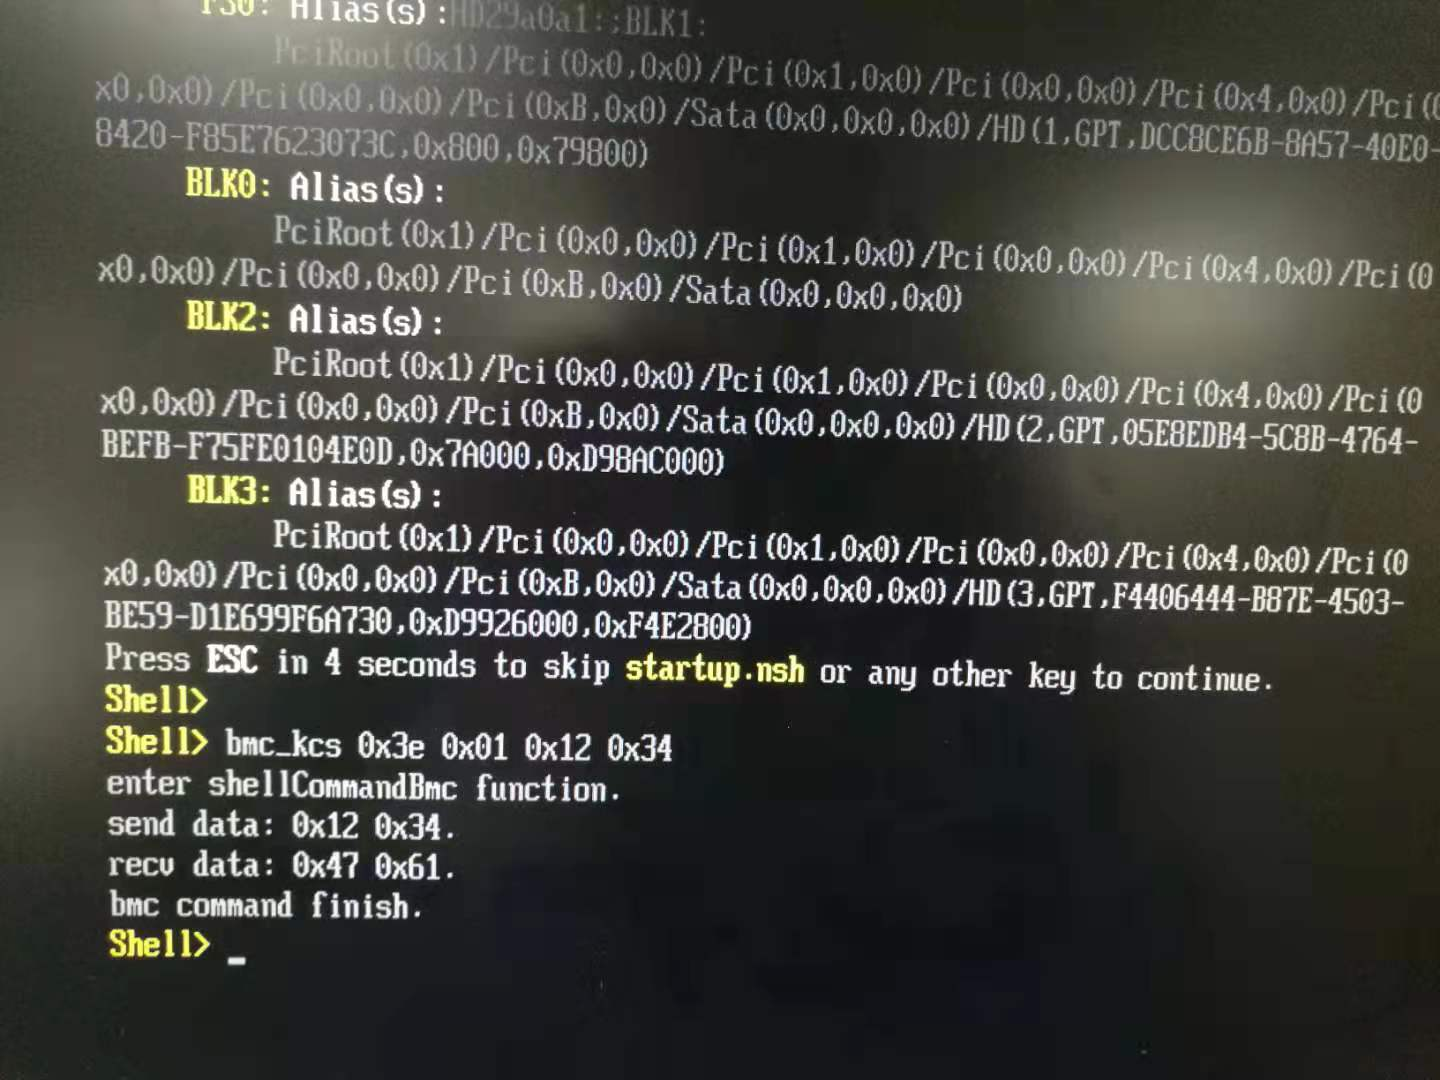
\includegraphics[width=12cm]{bmc_kcs.png}
    % 中文标题 %
    \caption*{图 5-7 BMC命令运行结果}
    % 调整图片英文标题与下文距离(本文标准为-0.7cm) %
    \setlength{\belowcaptionskip}{-0.7cm}
    % 英文标题 %
    \caption*{Figure 5-7 BMC command results}
\end{figure}

%
% 5.4节
%
\section{依赖表达式验证}

\subsection{测试目的}
依赖表达式是PEI和DXE驱动加载阶段的加载顺序的主要依据,他与优先级文件对应,属于弱类型。通过验证依赖表达式
在固件文件中的存储以及在驱动加载过程中如何控制加载顺序,可确保可信度量驱动在需被度量的特定驱动前加载,保证
度量功能的可用性。

\subsection{测试步骤}
(1)在DXE core代码的调度器程序中添加向SHELL输出的DEBUG函数。
\par (2)通过配置VS2008来对UEFI BIOS进行编译,得到NT32.fd文件。
\par (3)通过UEFITool这个fd文件解析程序,对NT32.fd进行解析。
\par (4)运行模拟程序的入口点exe可执行文件,根据SHELL输出的DEBUG信息得到依赖表达式解析过程。

\subsection{测试过程}
在经过VS2008编译器编译后生成Windows平台的UEFI模拟环境固件文件,通过UEFITool工具查看到的文件信息如下。

\begin{figure}[H]
    \label{ffs_format}
    % 调整图片与上文的垂直距离 %
    \vspace{0cm}   
    % 调整图片图片与中文标题、中文标题与英文标题距离 %
    \setlength{\abovecaptionskip}{0.3cm}
    % 引用/fig/目录中的图片文件 %
	\centering
    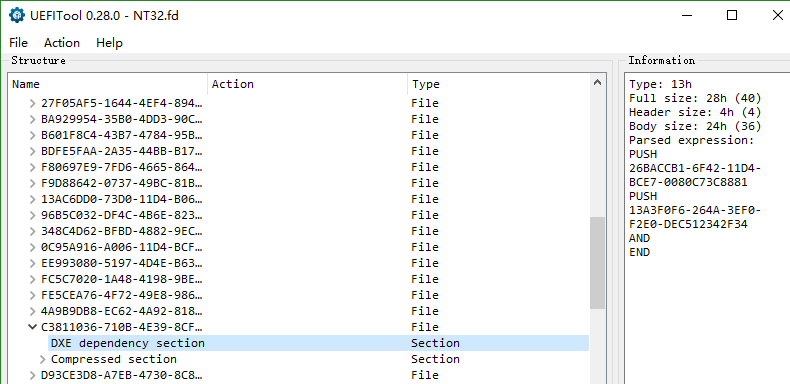
\includegraphics[width=12cm]{fd_depex.png}
    % 中文标题 %
    \caption*{图 5-8 固件文件依赖区域内容}
    % 调整图片英文标题与下文距离(本文标准为-0.7cm) %
    \setlength{\belowcaptionskip}{-0.7cm}
    % 英文标题 %
    \caption*{Figure 5-8 FD file dependency section content}
\end{figure}

图5-8所示的是DXE阶段的TimerDxe驱动在FV格式的固件卷中的dependency section中的内容,两个GUID分别代表两个
协议,他们对应的名称是gEfiCpuArchProtocolGuid和gEfiPcdProtocolGuid。下面是运行过程中TimerDxe驱动对应
的加载过程日志信息显示。

\begin{figure}[H]
    \label{ffs_format}
    % 调整图片与上文的垂直距离 %
    \vspace{0cm}   
    % 调整图片图片与中文标题、中文标题与英文标题距离 %
    \setlength{\abovecaptionskip}{0.3cm}
    % 引用/fig/目录中的图片文件 %
	\centering
    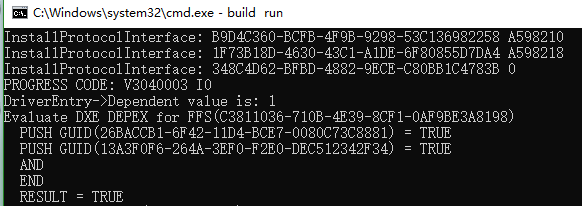
\includegraphics[width=12cm]{timer_depex.png}
    % 中文标题 %
    \caption*{图 5-9 驱动加载过程中的日志信息}
    % 调整图片英文标题与下文距离(本文标准为-0.7cm) %
    \setlength{\belowcaptionskip}{-0.7cm}
    % 英文标题 %
    \caption*{Figure 5-9 Log information during driver loading}
\end{figure}

图5-9显示的是在通过SecMain.exe入口点或命令build run执行后在windows终端里打印显示的BIOS运行过程中的日志
信息,其中可以看到入栈两个协议GUID的过程,并可以看出判断的最终结果为TRUE,在这段log的下方可看到显示了驱动
加载的日志信息。

%
% 5.6节
%
\section{本章小结}
通过三个实验过程的结果可以看出,可信度量驱动具备着从BMC取基准值、生成度量日志和根据依赖表达式定制驱动加载
顺序的功能,这些基本的功能也保证了安全方案的可实现性。

% \include{data/chap06}
% \include{data/chap07}
\chapter{实例章节}
\label{cha:introduction}

以下是简单的示例代码。
\par \textbf{加粗}[title=代码段题目]

\begin{lstlisting}
EFI_STATUS InfoRead(char *FileName,char *Buf)
{
    EFI_STATUS Status=0; //4个空格
    EFI_FILE_PROTOCOL *FileHandle=0; //4个空格
	EFI_FILE_PROTOCOL *RootHandle; //tab
  UNINT BufSize=10240; //2个空格
}
\end{lstlisting}

插入文本格式代码:
\\ void main() \{
\par return 0;
\par ASDFSJOGASJDIGOS;
\\ \}
\section{二级标题}

\subsection{三级标题}

\subsubsection{四级标题}

\paragraph{段落标题}

这是一段文字。

\section{公式}
\label{sec:equation}

% 在不需要引用时,\label可以省略
\begin{equation}
\label{eq:error}
	E_p=\sum_i\rho_h(e_{p,i}^T\Omega_i^{-1}e_{p,i})
\end{equation}
其中,$\rho_h$为Huber鲁棒代价函数,增加了系统对于噪声点的鲁棒性……
% 方程组使用\left\{\begin{aligned}\end{aligned}\right.
% 矩阵考虑\begin{array}\end{array}

\subsection{引用}

上角标引用:ORB算法\cite{ORB},LSD算法\tcite{LSD},ORB-SLAM2\cite{ORB-SLAM2}算法。非角标引用:基于多视角互补的SLAM算法\mcite{xs2020SLAM}。

\subsection{插图}

\subsubsection{figure}

插入图片。多幅图像排列时,使用subfigure或minipage。
% 图片位置参数:! 不考虑美学, h 当前位置, t 页面顶部, b 页面底部, p 独立一页(一般不用)
\begin{figure}[htb]
	\centering
	% includegraphics支持width、height、scale参数
	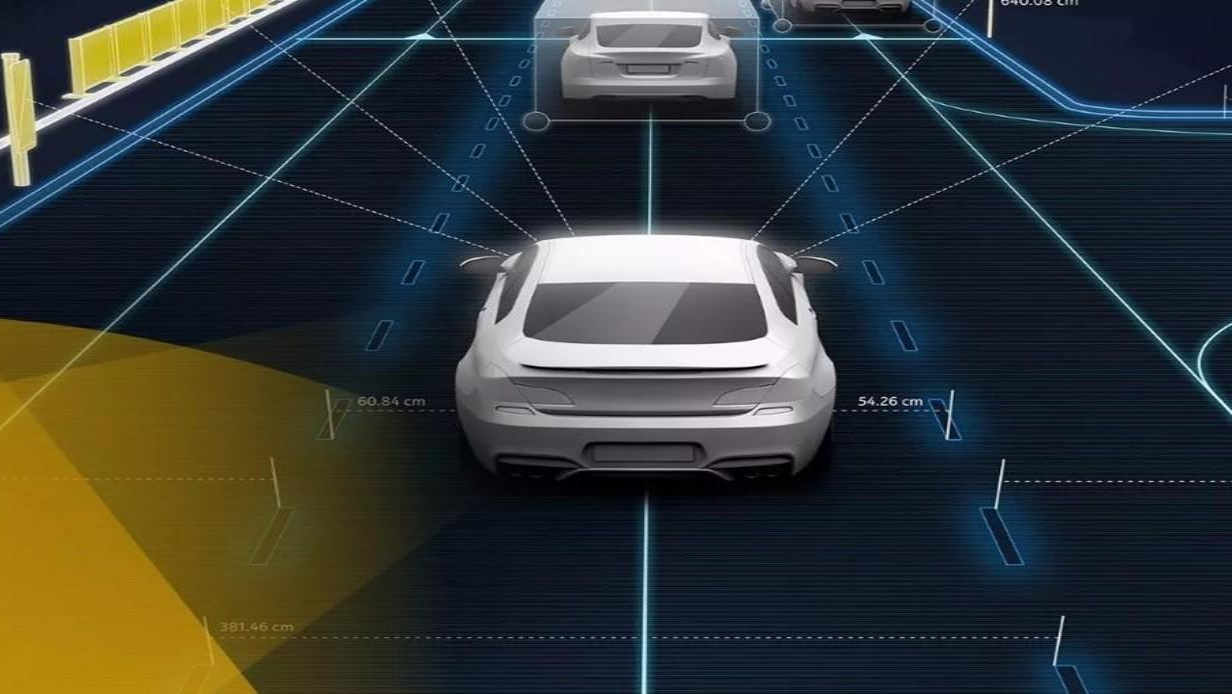
\includegraphics[width=0.7\textwidth]{autodrive.png}
	% footnotemark和footnotetext配合可以标注图片来源
	\caption{自动驾驶中的环境建模\protect\footnotemark[1]}
	\label{fig:introduction:autodrive}
	\addtocounter{figure}{-1}
	\renewcommand{\figurename}{Fig.}
	\caption{The environment reconstruction in automatic driving}
\end{figure}
\footnotetext[1]{图片来自于网络 http://auto.eastday.com/a/180720170248887.html}

\subsubsection{minipage}
minipage示例如图\ref{fig:line_optim:input}所示。

\begin{figure}[htb]
	\centering
	\begin{minipage}[t]{0.45\textwidth}
		\centering
		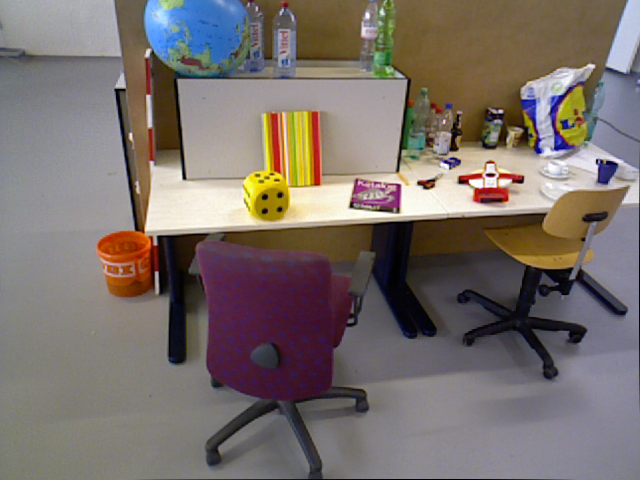
\includegraphics[width=0.8\textwidth]{tum-fr3-office-input1.png}
		\subcaption{场景输入图1}
		\label{fig:line_optim:input1}
	\end{minipage}
	\vspace{0.1in} %纵向间距,单位in或cm或pt等
	\begin{minipage}[t]{0.45\textwidth}
		\centering
		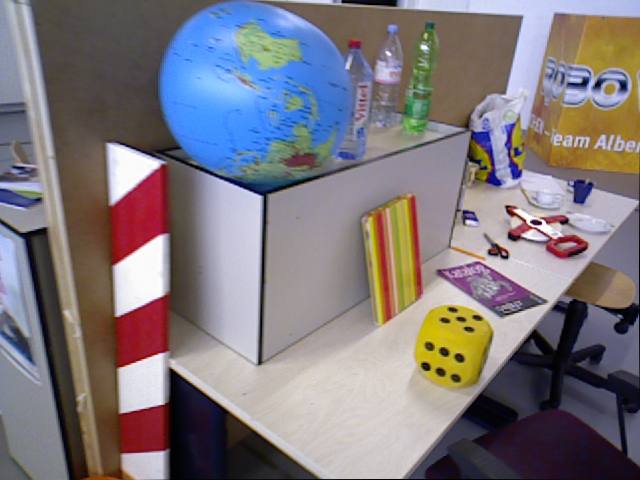
\includegraphics[width=0.8\textwidth]{tum-fr3-office-input2.png}
		\subcaption{场景输入图2}
		\label{fig:line_optim:input2}
	\end{minipage}
	\vspace{0.1in}
	\caption{TUM数据集{\itshape fr3\_long\_office}序列输入图}
	\label{fig:line_optim:input}
	\addtocounter{figure}{-1} %必须计数减一,否则上下中英标题的序号会递增
	\renewcommand{\figurename}{Fig.}
	\caption{The input images of {\itshape fr3\_long\_office} sequence in TUM dataset}
\end{figure}

\subsubsection{subfugure}
subfigure示例如图\ref{fig:line_optim:map}所示。

\begin{figure}[htb]
	\centering
	% subfigure[场景输入图像]{}
    \begin{subfigure}[b]{0.8\textwidth}
		\centering
		% 并排两个图像,也可以使用“\\”换行,改为纵向排列
        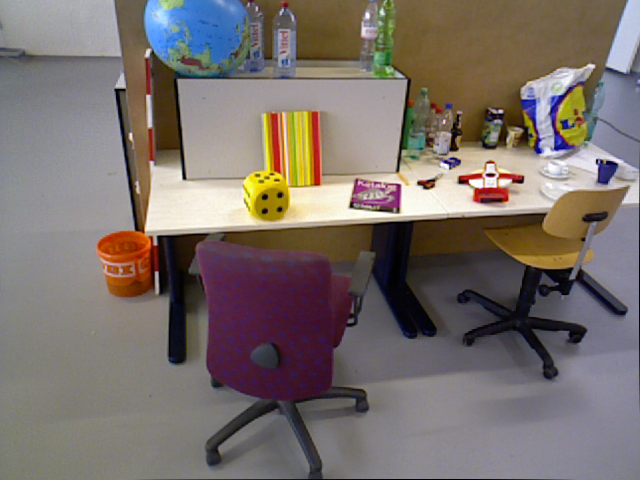
\includegraphics[width=0.45\textwidth]{tum-fr3-office-input1.png} %\\
        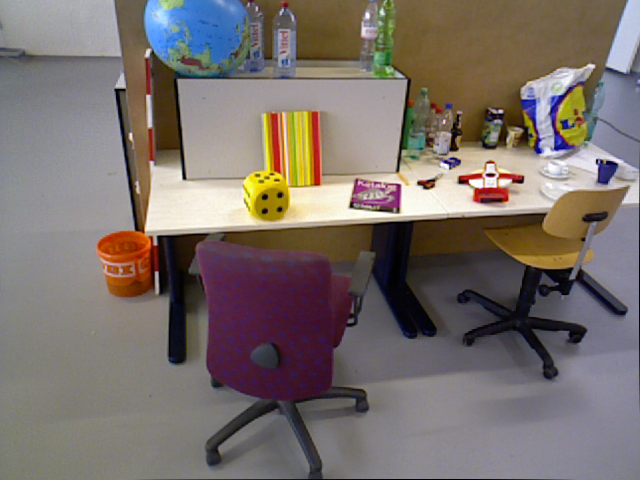
\includegraphics[width=0.45\textwidth]{tum-fr3-office-input1.png}
        \caption{场景输入图像}
    \end{subfigure}
    \vspace{0.3cm}
    \begin{subfigure}[b]{0.45\textwidth}
        \centering
        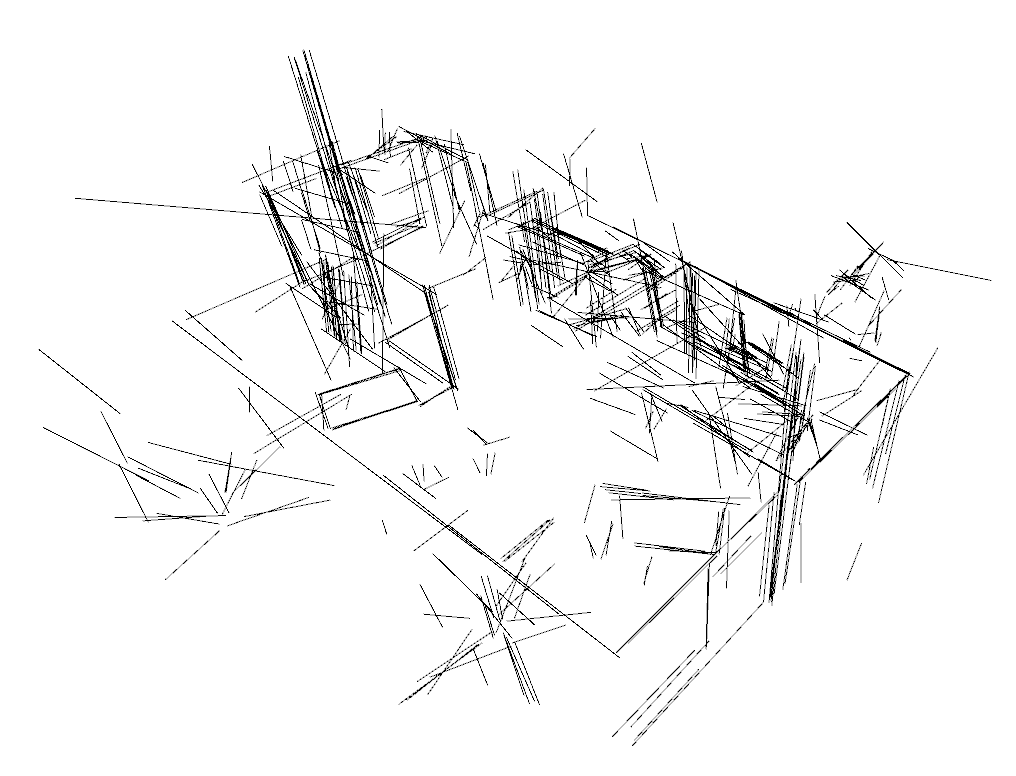
\includegraphics[width=0.9\textwidth]{line-map-TUM-fr3-office-lf.png}
        \caption{LF-SLAM算法的重建结果}
    \end{subfigure}
    \vspace{0.2cm}
    \begin{subfigure}[b]{0.45\textwidth}
        \centering
        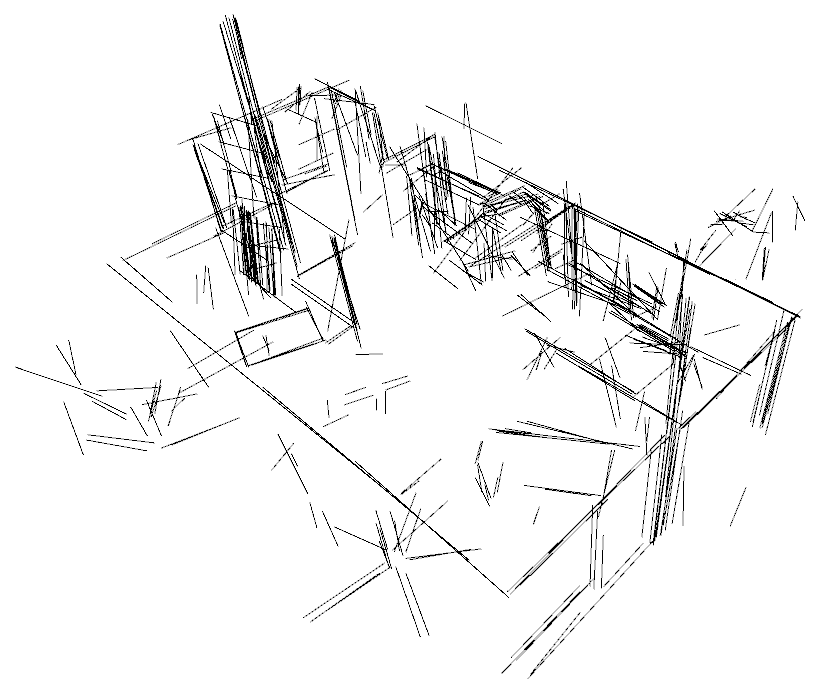
\includegraphics[width=0.9\textwidth]{line-map-TUM-fr3-office-ours.png}
        \caption{本章算法的重建结果}
    \end{subfigure}
    \vspace{0.2cm}
	\caption{在TUM {\itshape fr3\_long\_office}序列上的重建结果}
    \label{fig:line_optim:map}
    \addtocounter{figure}{-1}
    \renewcommand{\figurename}{Fig.}
    \caption{The results of mapping on {\itshape fr3\_long\_office} sequence in TUM}
\end{figure}

\subsection{表格}

tzz表格如111111111111111下所示:

\begin{table}[htb]
	\vspace{-0.5cm}                   %中文标题与上文距离
    \centering
	\small
	\setlength{\abovecaptionskip}{-0.3cm}
	\setlength{\belowcaptionskip}{0.3cm} 
	\caption*{test的表格}
	\caption*{test's table} 
	\begin{center}
		% c 居中,l 左对齐,r 右对齐,t 指定列宽,顶部对齐,b 底部对齐,p 指定列宽,顶部对齐, m 指定列宽,居中对齐
		% | 表格竖线
        \begin{tabular*}{\hsize}{@{}@{\extracolsep{\fill}}ccc@{}}
		\toprule[0.75pt]
		数据集	&ORB-SLAM	&PL-SLA	\\
        \midrule[0.5pt]
        TUMaaaaaaaaa			&20.6aaaaaaaaa 		&45.9cccccccc	\\
        7-Scenesaaaaaaa	&20.0bbbbbbbbbbb		&45.4ccccccccc	\\
		\bottomrule[0.75pt]
        \end{tabular*}
	\end{center}
	\vspace{-0.7cm}    %表格与下文距离
\end{table}
文字文字文字文字文字文字文字文字文字文字文字文字文字文字文字文字文字文字文字文字文字文字文字文字文字文字
文字文字文字文字文字文字文字文字文字。
\begin{table}[htb]
	\label{tab:parametervalues}
	\caption*{参数数值表}
	\caption*{Parameter values Table}
	\begin{tabular*}{\hsize}{@{}@{\extracolsep{\fill}}ccc@{}}
	\toprule[0.75pt]
	$p_{t}$  &21  &22\\
	\midrule[0.5pt]
	$c_{t}$aaaaaaaaaaaa  &EFI\_SIMPLE\_TEXT\_INPUT\_PROTOCOL*   &\makecell[c]{13caaaaaa\\aaaaaaaa\\cccc}\\
	$h_{t}$aaaaaaaaaaaa  &10bbbbbbbbb  &5ccccccccc\\
	\bottomrule[0.75pt]
	\end{tabular*}
	\vspace{-0.3cm}    %表格与下文距离
\end{table}
文字文字文字文字文字文字文字文字文字文字文字文字文字文字文字文字文字文字文字文字文字文字文字文字文字文字
文字文字文字文字文字文字文字文字文字。文字文字文字文字文字文字文字文字文字文字文字文字文字文字文字文字文字文字文字文字文字文字文字文字文字文字
文字文字文字文字文字文字文字文字文字。文字文字文字文字文字文字文字文字文字文字文字文字文字文字文字文字文字文字文字文字文字文字文字文字文字文字
文字文字文字文字文字文字文字文字文字。文字文字文字文字文字文字文字文字文字文字文字文字文字文字文字文字文字文字文字文字文字文字文字文字文字文字
文字文字文字文字文字文字文字文字文字。文字文字文字文字文字文字文字文字文字文字文字文字文字文字文字文字文字文字文字文字文字文字文字文字文字文字
文字文字文字文字文字文字文字文字文字。文字文字文字文字文字文字文字文字文字文字文字文字文字文字文字文字文字文字文字文字文字文字文字文字文字文字
文字文字文字文字文字文字文字文字文字。
\subsection{列表}

\subsubsection{enumerate}
enumerate列表带编号,默认样式1.

\begin{enumerate}[(1)]
	\item 分析现有SLAM框架的优势和不足,提出一种多视角互补的SLAM框架,该框架对现有框架做了改进,相比于现有框架,利用了观测数据的帧间约束信息,在位姿精度和重建效果方面提供了更大的提升空间。
	\item 在多视角互补框架下,结合多视角观测信息,提出一种可信度量方式,尽可能地降低不可靠特征对位姿优化带来的干扰,提升相机定位精度。
	\item 在多视角互补框架下,利用前后帧的观测信息,求解相机位姿和三维特征信息,同时也对局部帧的二维线条进行反向优化,提升线条完整度和端点的准确度,从而提升重建质量。
	\item 在多视角互补框架下,融合点线面特征,构建复合特征,在复合特征结构下,优化求解相机位姿和三维地图,提升优化速度和位姿精度,提高地图重建质量。 
\end{enumerate}

\subsubsection{itemize}
itemize列表

\begin{itemize}
\item 第1章\quad 绪论

\item 第2章\quad 相关知识及数据集

\item 第3章\quad 基于多视角互补的SLAM框架

\item 第4章\quad 基于多视角互补的捆绑优化算法

\item 第5章\quad 基于多视角互补的线条优化算法

\item 第6章\quad 基于多视角互补的复合特征优化算法

\item 结论

\end{itemize}

\bjutclearpage
\begin{APP}
UEFI文件系统协议栈作为UEFI系统环境中和硬盘设备硬件之间的桥梁,是一个保证硬盘ESP分区中数据信息不被从固件层面
攻击的关键环节。UEFI文件系统协议栈在负责BIOS系统与硬盘设备间进行数据交互的同时,也作为一个UEFI系统启动中DXE
阶段的一些驱动程序的形式进行向系统中的集成与加载。由于硬盘ESP分区中数据文件的重要性,以及近年来越来越多的硬件
攻击手段的出现,不仅有针对硬盘设备的攻击也存在针对固件芯片的攻击,基于这种情况,本为设计了基于UEFI的硬盘文件
安全加载的策略,在一定程度上保证了计算机通过UEFI BIOS和硬盘设备启动过程中的安全性。
\par 本文的主要工作内容总结归纳如下:
\par 1.针对UEFI BIOS系统加载硬盘文件过程中存在的安全威胁,分析目前基于UEFI系统的服务器在通过硬盘ESP
分区中操作系统引导文件启动的加载过程中的安全漏洞,即硬盘设备和固件芯片设备两个可被攻击的对象结合可信计算理论
提出基于UEFI的硬盘设备文件可信加载系统的总体框架,并使用的底层可信平台BMC及基板管理控制器,实现UEFI BIOS中
BMC驱动程序。
\par 2.针对UEFI BIOS系统加载UEFI BIOS存储闪存设备中的驱动文件过程中存在的安全问题,设计提出UEFI BIOS启动
阶段所需度量的UEFI文件系统协议栈驱动程序,并实现度量模块功能。
\par 3.针对安全方案中的可信度量功能,设计并实现了通过BMC的日志存储功能,并完成确保驱动按顺序加载的依赖表达式
编写。由于需要在被度量驱动前先加载可信度量驱动,因此存在DXE阶段调度程序加载驱动顺序的问题,通过UEFI中的依赖表
达式来完成这一要求,保证度量过程的可实施性。
\par 4.根据本系统安全方案的设计,在申威平台中对驱动度量模块、日志生成功能和驱动加载
顺序修改功能进行实现和测试,以保证功能开发过程的有效性和安全方案的可实施性。
% \par 1.对UEFI系统启动阶段和UEFI文件系统协议栈相关驱动进行研究,分析目前基于UEFI系统的服务器在通过硬盘ESP
% 分区中操作系统引导文件启动的加载过程中的安全漏洞,即硬盘设备和固件芯片设备两个可被攻击的对象,结合可信计算
% 思想,提出了服务器计算机安全加载硬盘文件的策略。
% \par 2.安全方案中驱动度量模块的设计。驱动度量模块设计为DXE阶段的可信度量驱动中的一个内容,他是负责在所有
% DXE调度程序加载的驱动中检索出文件系统协议栈相关的驱动程序的关键,他通过GUID的方式筛选出需要度量的特定驱动,
% 以达到自定义度量驱动程序的目的。度量模块是整个可信驱动的关键部分,由他来调度度量值计算模块和基准值取出功能,
% 最终形成一个可信度量的结果。其中还包括了申威平台特有的向BMC写入日志信息的过程,作为可信度量驱动中日志形成
% 的实现方法。由于PEI阶段和DXE阶段的系统函数不同,而可信度量驱动都需要进行系统调用,因此设计两个阶段单独的
% 度量驱动以供安全方案使用。由于需要在被度量驱动前先加载可信度量驱动,因此存在DXE阶段调度程序加载驱动顺序的
% 问题,通过UEFI中的依赖表达式来完成这一要求,保证度量过程的可实施性。
% \par 3.UEFI可信启动信任链的设计。信任链的设计与实现是最终在BDS阶段UEFI系统能安全加载硬盘文件的基础,他从
% SEC阶段起始,通过设计的BMC可信平台模块来代替传统TPM模块进行信任链的传递。SEC、PEI、DXE、BDS阶段分别设计
% 使他们度量下一阶段的核心代码,并根据每个阶段的流程特点,制定出具体的驱动加载和度量方法。其中SEC和PEI阶段
% 作为开始和中间阶段,由DXE和BDS阶段分别负责UEFI文件系统协议栈驱动程序和硬盘文件的度量,以保证安全方案的可
% 实施性。
% \par 4.UEFI BIOS中BMC驱动程序的设计。BMC驱动程序是安全方案中度量驱动程序和硬盘文件数据的关键,由他负责取出
% 存储在BMC芯片中的驱动和文件基准值,来进行度量。BMC驱动分为PEI和DXE阶段两个,文中主要对DXE阶段的BMC驱动介绍
% 的原因也在于在实验的真机环节中,UEFI启动阶段受到定制,去掉了PEI阶段,只存在DXE阶段的可信度量驱动的加载,但
% PEI阶段作为UEFI规范中的一个环节,因此安全方案也对这一阶段做出了设计内容。BMC驱动需要符合IPMI协议,并通过KCS
% 接口来进行BMC系统的访问,数据的输入和输出流程符合IPMI协议规范以及BMC相关寄存器的使用方法。
% \par 5.对安全方案中的关键模块功能进行验证,验证的实验环节也分为真机环节和edk基础版本相同的Windows模拟环境
% 来进行。其中模拟环境的设置有助于CPU体系结构不相关的功能模块的开发效率,在通过模拟环境的编译和测试后,再进行
% 真机环境的验证。
\par 综上所述,本方案解决了UEFI系统在加载硬盘文件时容易收到硬盘设备和固件芯片两方面攻击的问题,并给出了UEFI
启动阶段中度量的具体内容和具体方式,保证了UEFI环境中加载硬盘文件的安全可信。但本方案也存在着很多不足之处和
需要进一步改进的地方,在于:
\par 1.目前可信度量的过程在UEFI BIOS环境中完成,但根据可信平台模块的基本功能,度量的过程应由平台模块来进行,
也就是可以改进为通过BIOS发送在固件和硬盘中加载的特定驱动和文件的数据内容,通过BMC驱动发送给BMC中的可信平台
模块,由BMC系统进行度量值的计算和日志生成过程,并将度量结果返回给BIOS,BIOS通过结果来判断下一步的执行安排。
\par 2.目前的度量日志的内容只能通过操作系统中的BMC维护程序来获取,可进一步在UEFI BIOS环境中编写获取BMC系统
中存放的日志内容的功能,可从UEFI SHELL环境中获取日志信息,使功能更加完善。

\end{APP}

%\bjutclearpage
%\chapter{攻读硕士学位期间发表的学术论文}
%\label{cha:seven_achievements}
\begin{APP2}
\begin{enumerate}

    \item 张建标,唐治中,张恒等. 一种基于基础性的UEFI BIOS固件系统中驱动程序的保护方法.发明专利.专利号/申请号:202110121999.5.
    
\end{enumerate}
\end{APP2}

\bjutclearpage

\backmatter

%
% 参考文献
%
\bibliographystyle{bjutthesis}
\bibliography{ref/refs}
\bjutclearpage

%
% 致谢
%
% 如果使用声明扫描页,将可选参数指定为扫描后的 PDF 文件名,例如:
% \begin{acknowledgement}[scan-statement.pdf]
\begin{acknowledgement}

时光荏苒,三年的研究生生活即将结束,研究生以及全部的在学校的学习生活也要告一段落,十分幸运有机会能够在北
工大信息学部进行三年的学习生活,这里的校园环境、同学氛围都是那么美好和值得怀念。在这里我不光学习到了书本
上的知识,也认识了在学习和生活中向我树立榜样的导师,也有共同学习奋斗的同学们,让我的研究生生活更加充实,
充满活力。在临近毕业之际,我要向曾不断给予我鼓励和帮助的导师、家人和同学致以诚挚的感谢!
\par 首先要向我的研究生导师张建标教授表示诚挚的感谢,在研究生阶段,有幸参加了张老师的底层系统项目,有机会
接触到了以前充满未知的底层系统,这也成为了我学习和研究的兴趣所在,通过项目的进行,从一开始的漫然无知,到
熟练操作项目中的各个环节,到阅读和学习底层系统的源码并加以更改添加可信功能,我很幸运的学习到了自己所感
兴趣的计算机领域,也丰富了自己的知识和实际解决问题的能力。除了学习上对我的帮助外,张老师在项目中也给了我
很多的实践学习机会,让我感受到了在社会中学习工作的不易,增加了我很多方面的经验。再次感谢张老师对我的指导
和栽培,希望在以后的工作生活中取得更多的进步。感谢信息安全的所有老师们,很荣幸能受到您们的指导,给我的学习
道路指引了方向。
\par 同时也要感谢实验室里的所有师兄们,你们在帮助我适应研究生生活的同时,也给予了我学习和生活上的帮助,
帮助我分析项目中的问题,找到解决问题的思路和技术方案,帮助我解决了一个又一个项目和学习中的困难。感谢我的
同届的实验室同学们,十分珍惜和你们的朝夕共处,一起的努力学习让我们有了更深厚的感情,让研究生生活变得更加
趣味横生、多姿多彩。感谢我的师弟师妹们,能够成为我学习道路上一起进取的伙伴,你们的陪伴让我更加珍惜学生时代
的美好时光。
\par 感谢我的室友们对我的照顾和陪伴,在学习和项目中遇到迷茫之时,你们总能给我带来很多的慰藉,让我总能够
重整心态,继续启航。希望我们的友谊能够继续长存,希望在今后的工作中能有更多的交流沟通机会。感谢所有和我一起
学习过生活过的挚友们,你们的陪伴让我在学习的路上不再孤单。
\par 感谢我的父母和家人,在我遇到困难和困苦时给我无限的鼓励,让我知道只有通过改变自己的方式,才能在不光
是工作和学习中、也在生活的方方面面取得突破,不断成长。
\par 最后,由衷的感谢参与评阅论文的所有老师们!

% \mbox{}
% \begin{flushright}
%     \parbox[]{2.8cm}{谢帅}\\
%     \parbox[]{4.5cm}{二零二零年五月于北京}
% \end{flushright}


\end{acknowledgement}


\end{document}
